% Main page
\documentclass[12pt]{article}
\renewcommand{\familydefault}{\sfdefault}
\usepackage[T1]{fontenc}
\usepackage[utf8]{inputenc}
\usepackage{enumitem}
\usepackage{graphicx}
\usepackage{helvet}
\usepackage{minted}
\usepackage{svg}
\usepackage{float}
\usepackage{hyperref} 

\begin{document}

% Title page
\begin{titlepage}
  \centering
  % \includesvg[width=0.5\textwidth]{react.svg}
  % \vspace{1cm}\\
  {\Huge\bfseries Programowanie zaawansowane II\par}
  \vspace{1cm}
  {\Large\itshape Ćwiczenia\par}
  \vfill
  {\large\itshape \begin{flushright}Igor Barcik 131780\par\end{flushright}}
  {\today\par}
\end{titlepage}
\tableofcontents \newpage
% 1
\section{Budowanie nowej aplikacji w Angular}
\begin{description}[leftmargin=.5em]
  \item Krok 1: Przygotowanie środowiska
  \item{\begin{itemize}
          \item Upewnij się, że masz zainstalowanego \textit{Node.js} na swoim komputerze.
          \item Zainstaluj narzędzie \textbf{Angular CLI} globalnie za pomocą polecenia \texttt{npm install -g @angular/cli}.
        \end{itemize}}
  \item Krok 2: Utworzenie nowego projektu Angular
  \item{\begin{itemize}
          \item Utwórz nowy projekt Angular, wykonując polecenie \texttt{ng new nazwa-projektu}. Postępuj zgodnie z instrukcjami w konsoli.
        \end{itemize}}
  \item Krok 3: Rozwinięcie projektu
  \item{\begin{itemize}
          \item Przejdź do katalogu projektu, wykonując \texttt{cd nazwa-projektu}.
          \item Twórz komponenty, usługi i edytuj szablony, aby dostosować projekt do swoich potrzeb.
        \end{itemize}}
  \item Krok 4: Uruchomienie aplikacji
  \item{\begin{itemize}
          \item Uruchom aplikację za pomocą polecenia \texttt{ng serve}.
        \end{itemize}}
  \item Krok 5: Testowanie i rozwijanie
  \item{\begin{itemize}
          \item Kontynuuj rozwijanie aplikacji, testowanie i dostosowywanie jej do swoich potrzeb.
        \end{itemize}}
\end{description}
% Image 1
\begin{figure}[H]
  \centering
  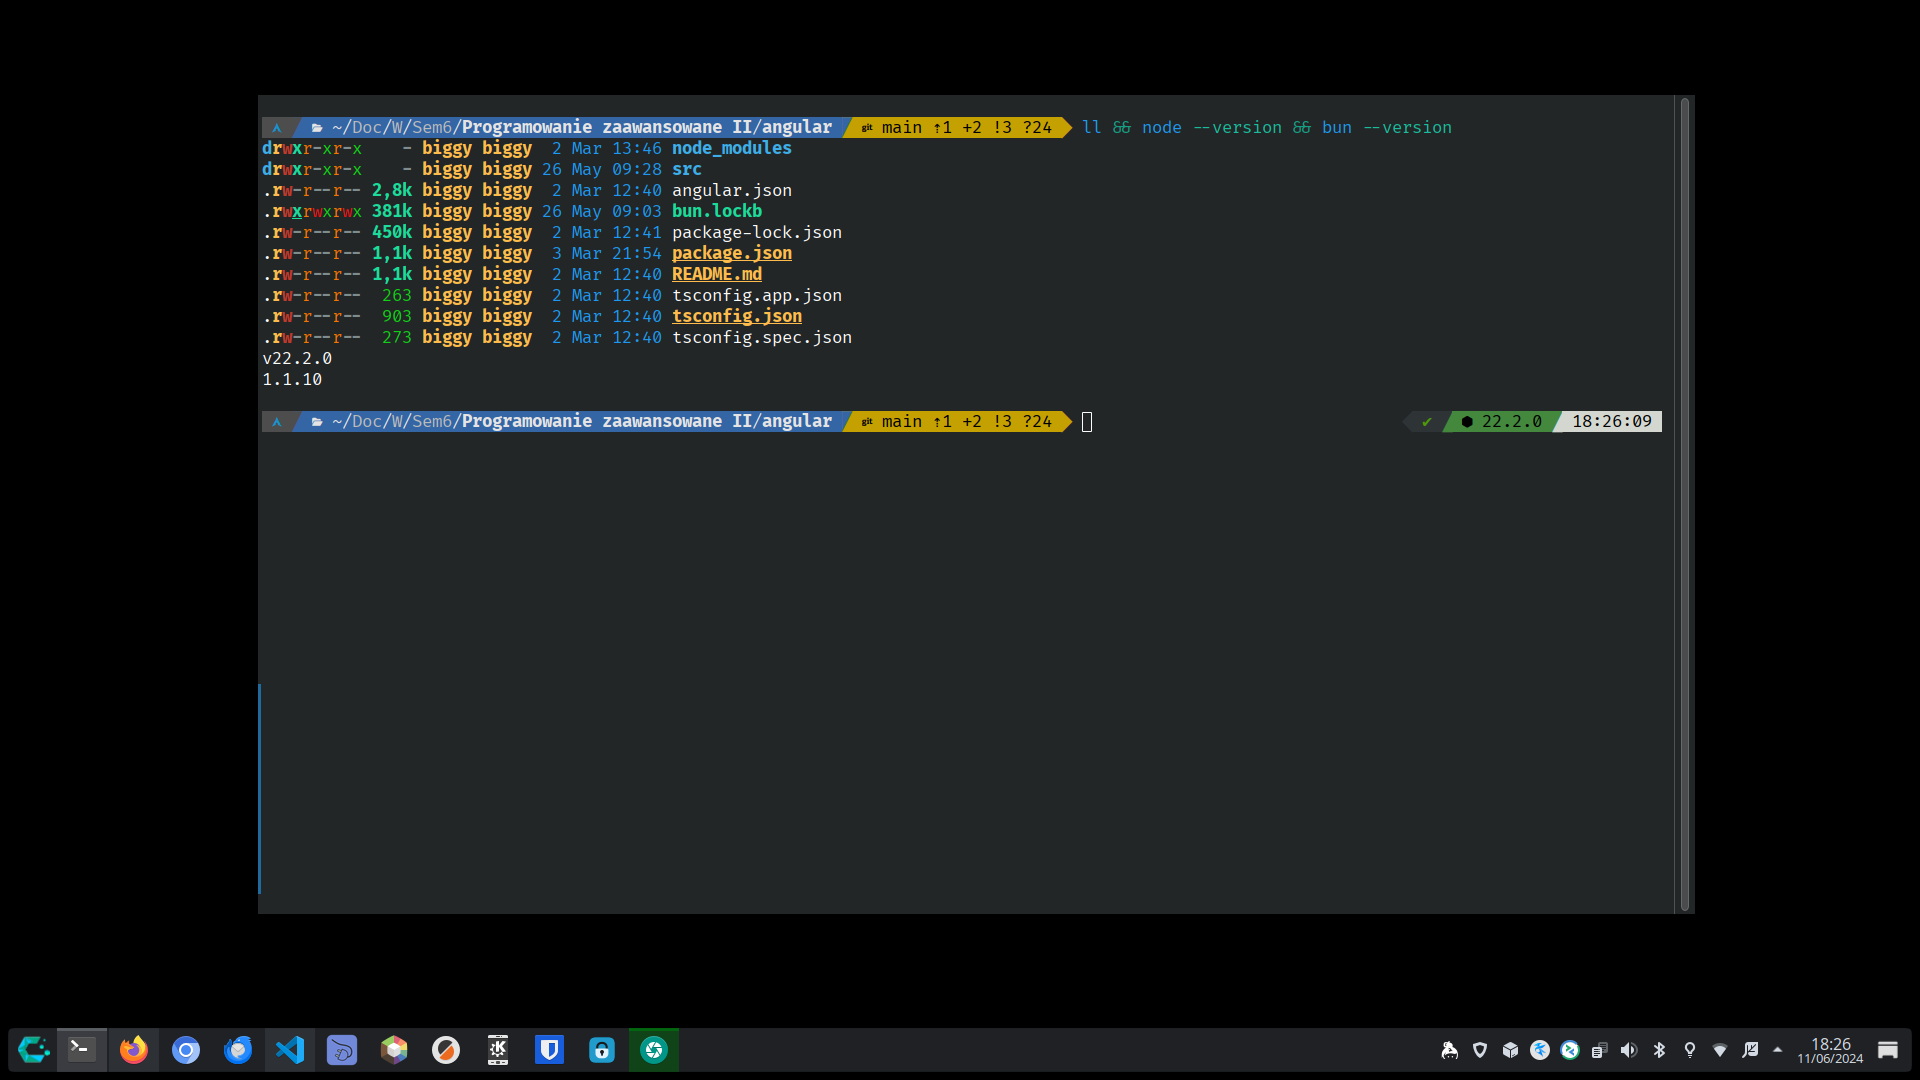
\includegraphics[width=1\textwidth]{image-2.png}
  \caption{Przygotowane środowisko, node v22.2.0, bun v1.1.10.}
  \label{fig:image-2}
\end{figure}

% 1.1
\subsection{Dodanie logowania}
\begin{description}[leftmargin=.5em]
  \item Krok 1: Utworzenie ekranu logowania
  \item{\begin{itemize}
          \item W terminalu przejdź do katalogu projektu za pomocą \texttt{cd nazwa-projektu}.
          \item Utwórz komponent logowania za pomocą Angular CLI: \texttt{ng generate component logowanie}.
          \item Edytuj plik \texttt{login.component.html}, aby utworzyć formularz logowania.
          \item W pliku \texttt{login.component.ts} zaimplementuj funkcję logowania.
        \end{itemize}}
  \item Krok 2: Uruchomienie aplikacji
  \item{\begin{itemize}
          \item Uruchom aplikację za pomocą polecenia \texttt{ng serve}.
          \item Twoja aplikacja będzie dostępna pod adresem \texttt{http://localhost:4200/}.
        \end{itemize}}
  \item Krok 3: Testowanie i rozwijanie
  \item{\begin{itemize}
          \item Kontynuuj rozwijanie aplikacji, dodawaj nowe funkcjonalności i testuj je.
          \item Monitoruj jakość kodu i utrzymuj projekt w dobrej kondycji.
        \end{itemize}}
\end{description}
%login.component.html
\subsubsection{\texttt{login.component.html}}
Zaprojektowanie prostego formularza logowania zawierającego pola \textit{login} i \textit{password}.
Zawiera również bloki z komunikatami o błędach. Całość wystilizowana odrobiną SCSS'a.
\begin{figure}[H]
  \centering
  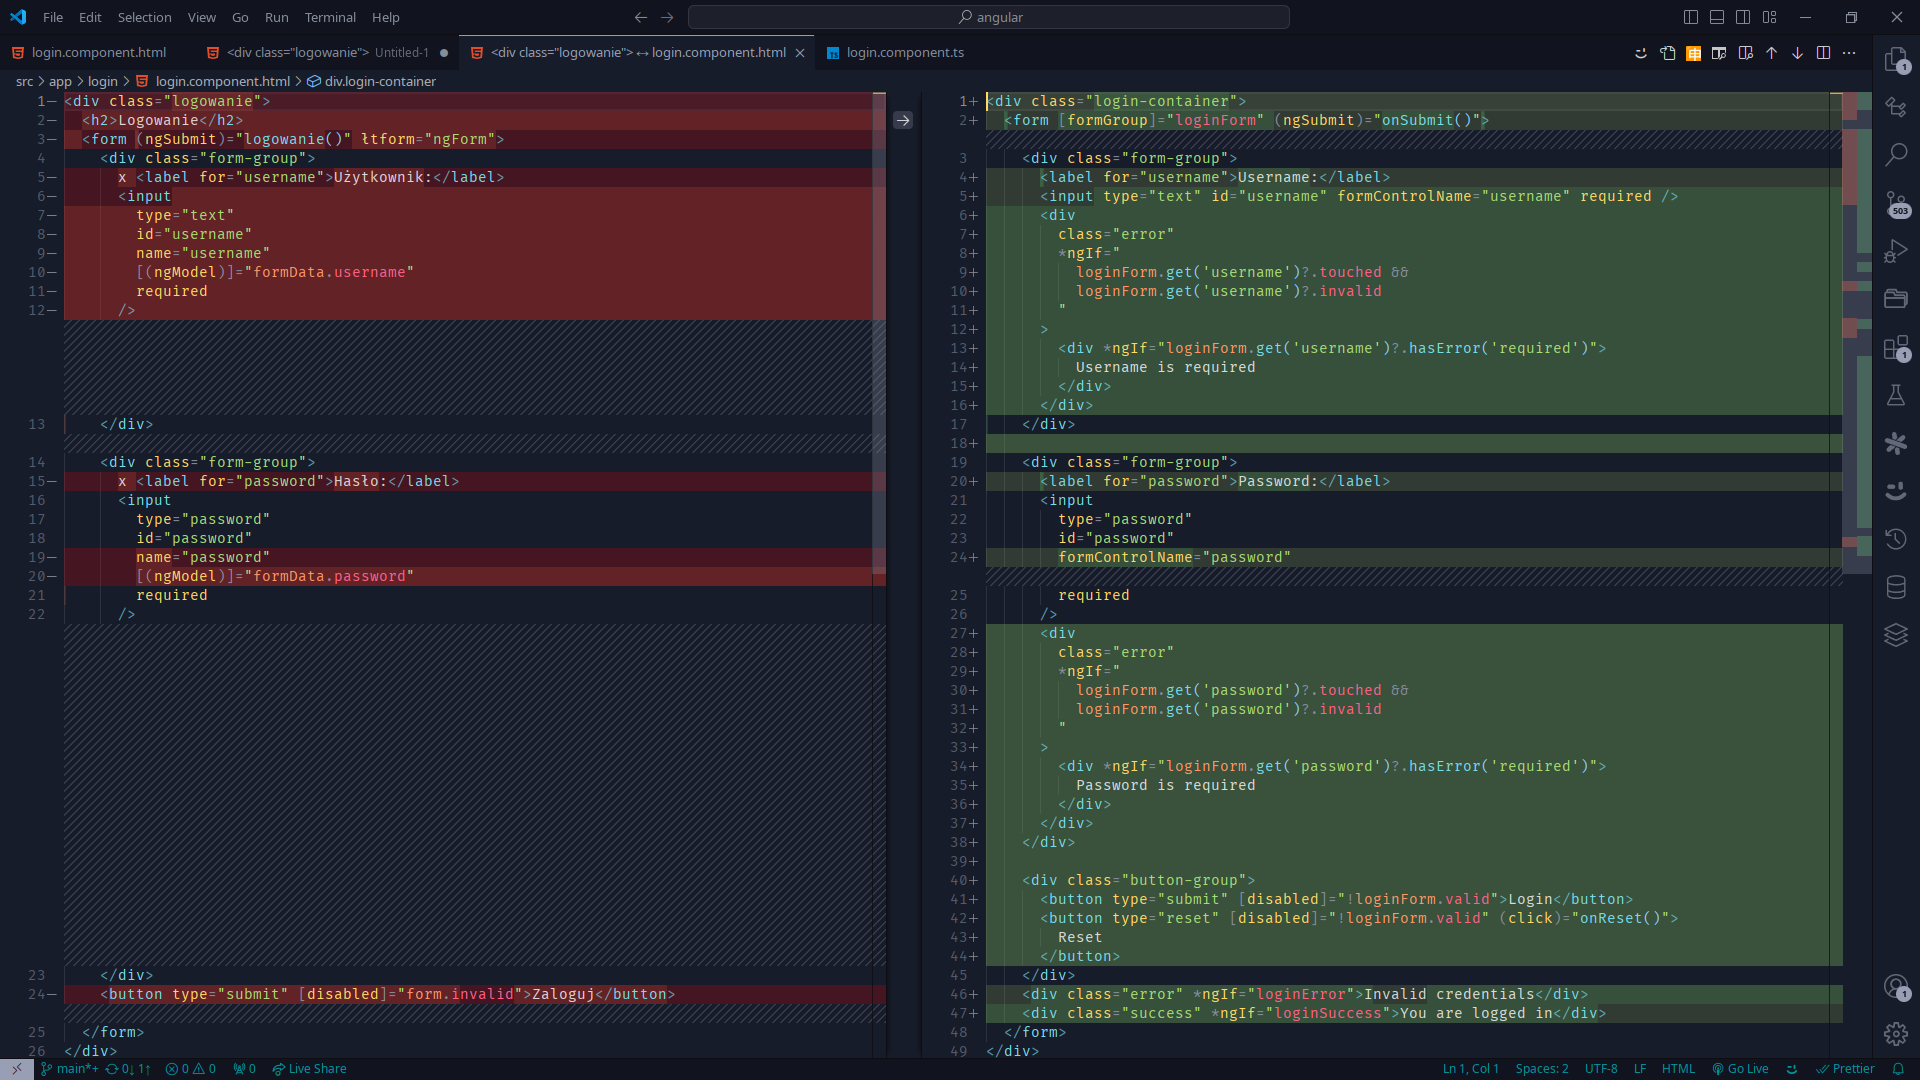
\includegraphics[width=1\textwidth]{image-4.png}
  \caption{Różnice między proponowanym rozwiązaniem a zaimplementowanym \texttt{login.component.html}}
  \label{fig:image-4}
\end{figure}
\begin{figure}[H]
  \centering
  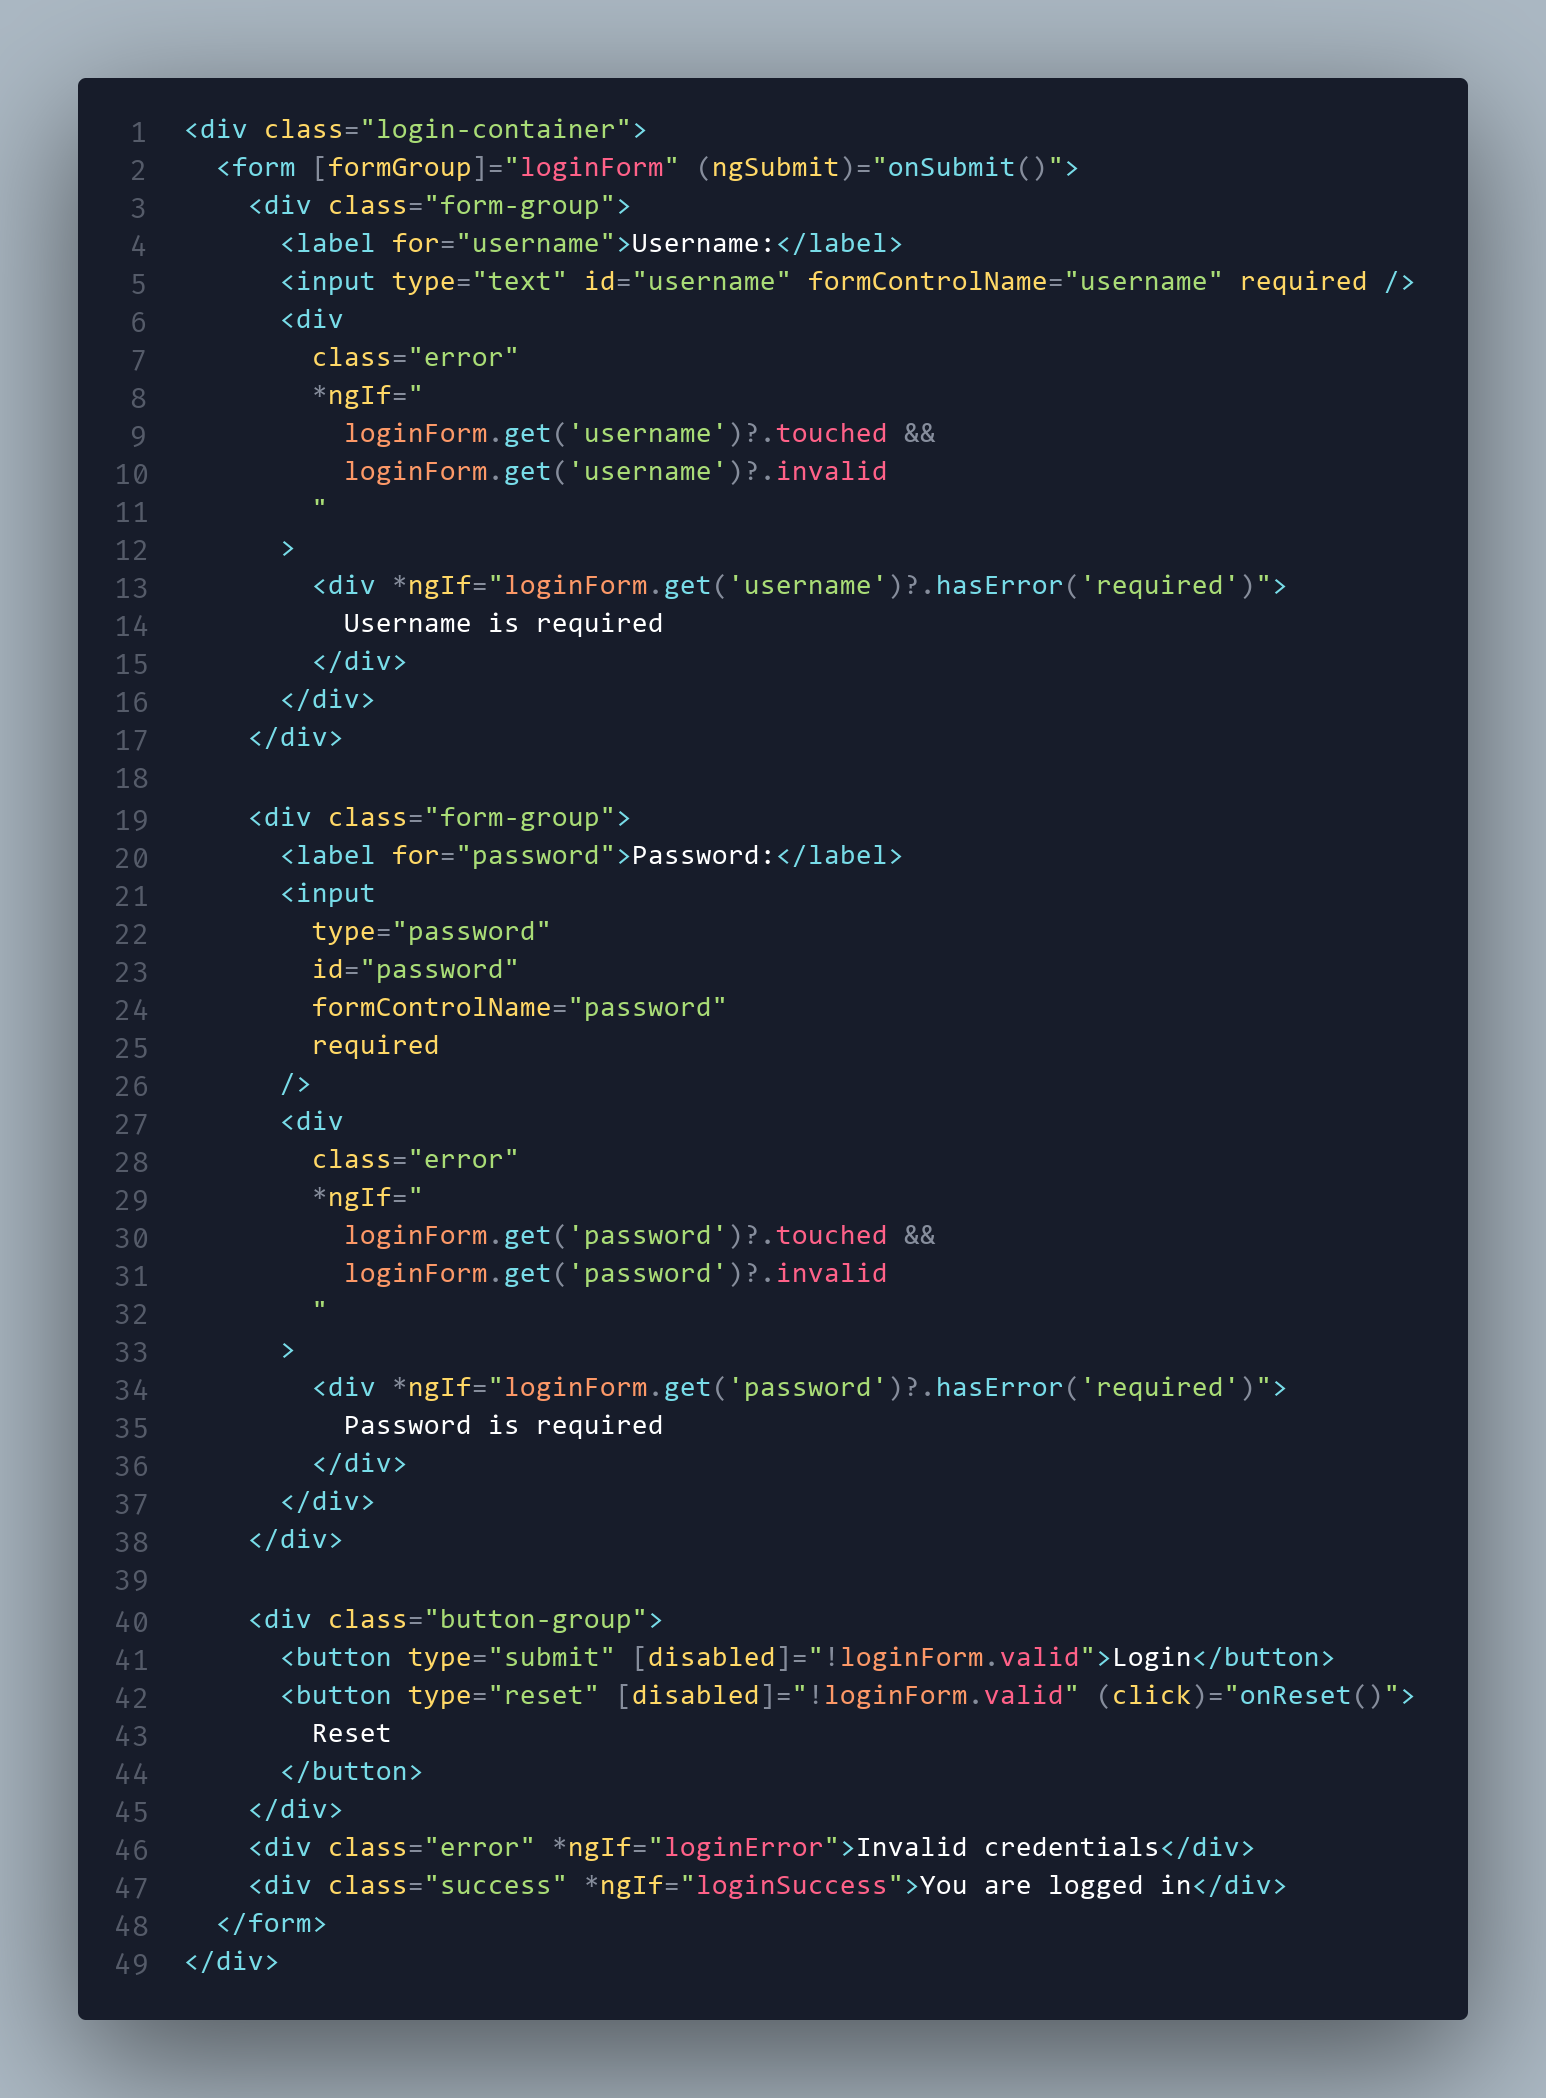
\includegraphics[width=1\textwidth]{image-5.png}
  \caption{Zaimplementowany \texttt{login.component.html}}
  \label{fig:image-5}
\end{figure}
%login.component.scss
\subsubsection{\texttt{login.component.scss}}
\begin{figure}[H]
  \clearpage
  \centering
  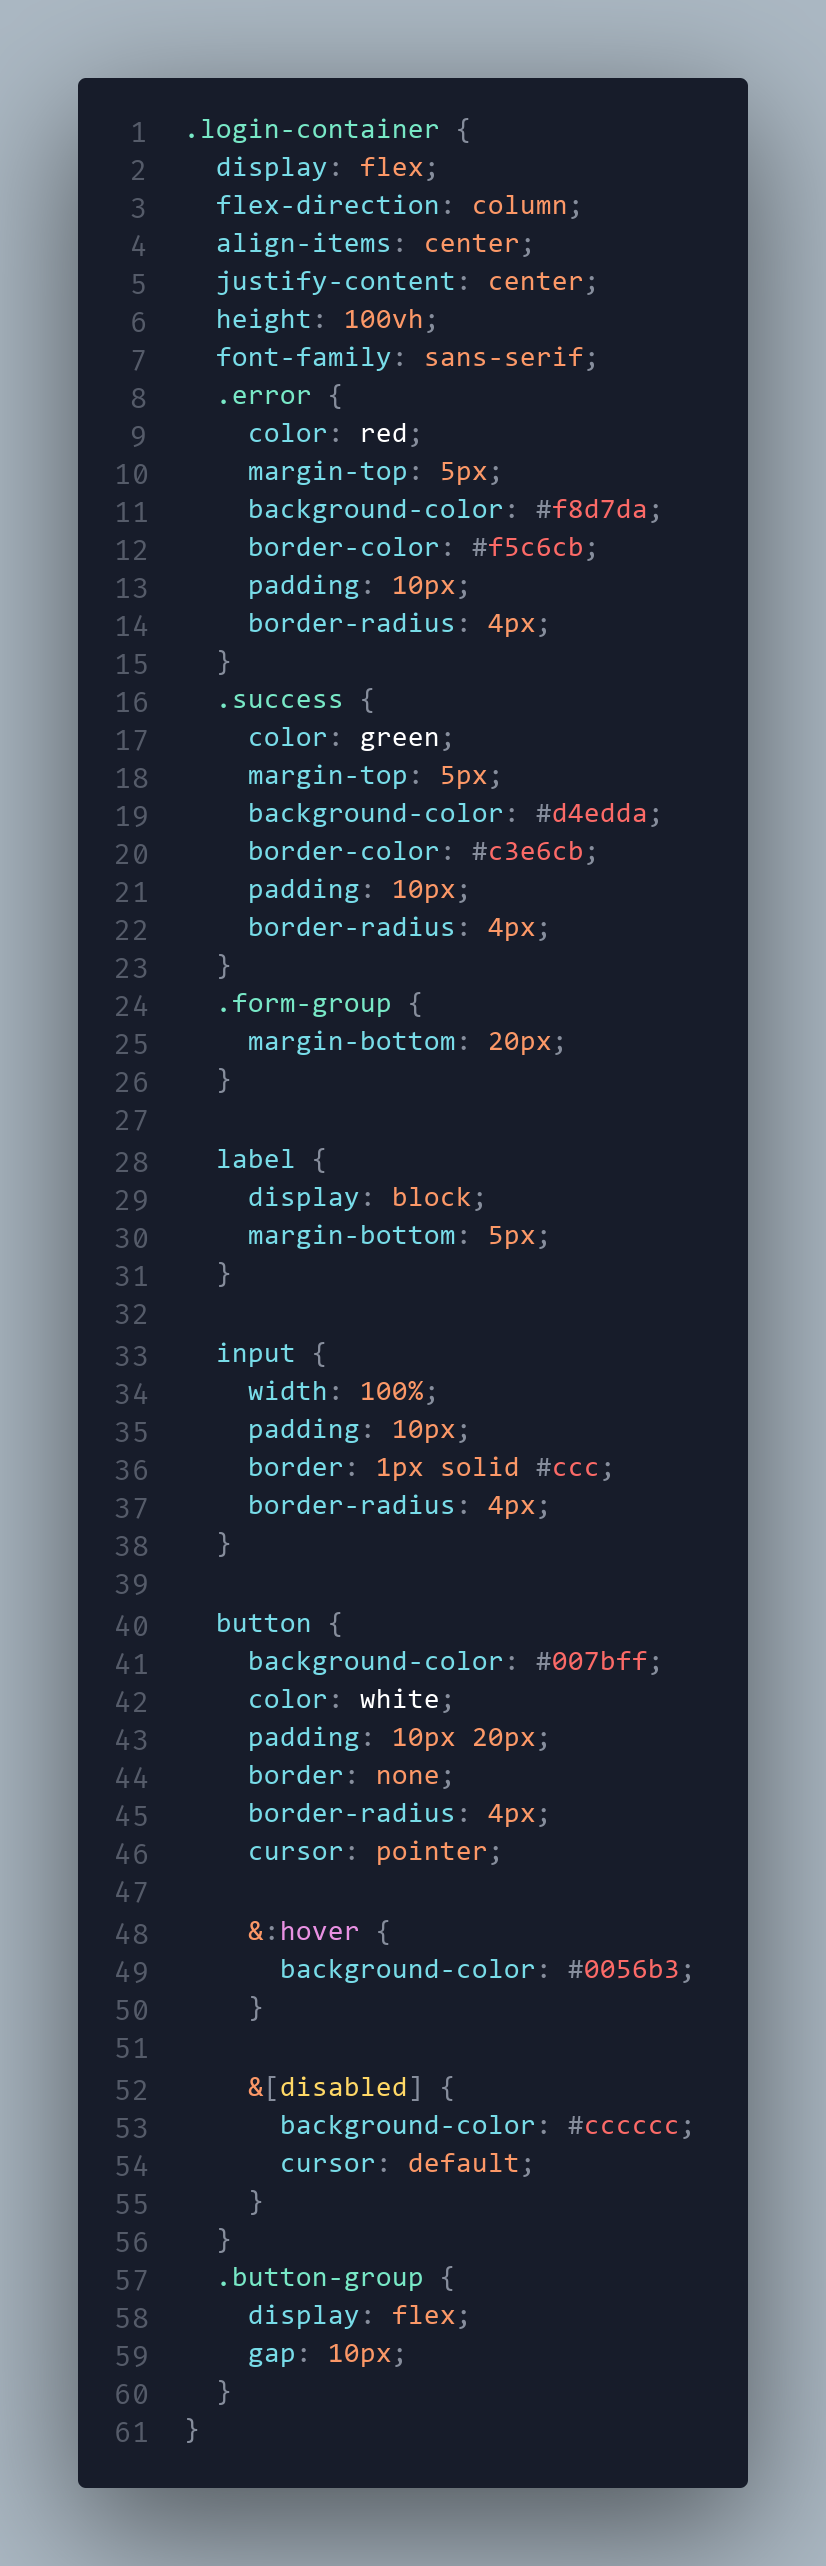
\includegraphics[height=\textheight]{image-6.png}
  \caption{Zaimplementowany \texttt{login.component.scss}}
  \label{fig:image-6}
\end{figure}
%login.component.ts
\subsubsection{\texttt{login.component.ts}}
Zawarcie prostej logiki komponentu logowania gdzie zwraca informacje o logowaniu do aplikacji wcześniej weryfikując dane wprowadzone przez użytkownika w komponencie serwisowym \texttt{auth.service.ts}.

\textit{Wzorowanie się na proponowanym rozwiązaniu załączonym przez prowadzącego.}
\begin{figure}[H]
  \centering
  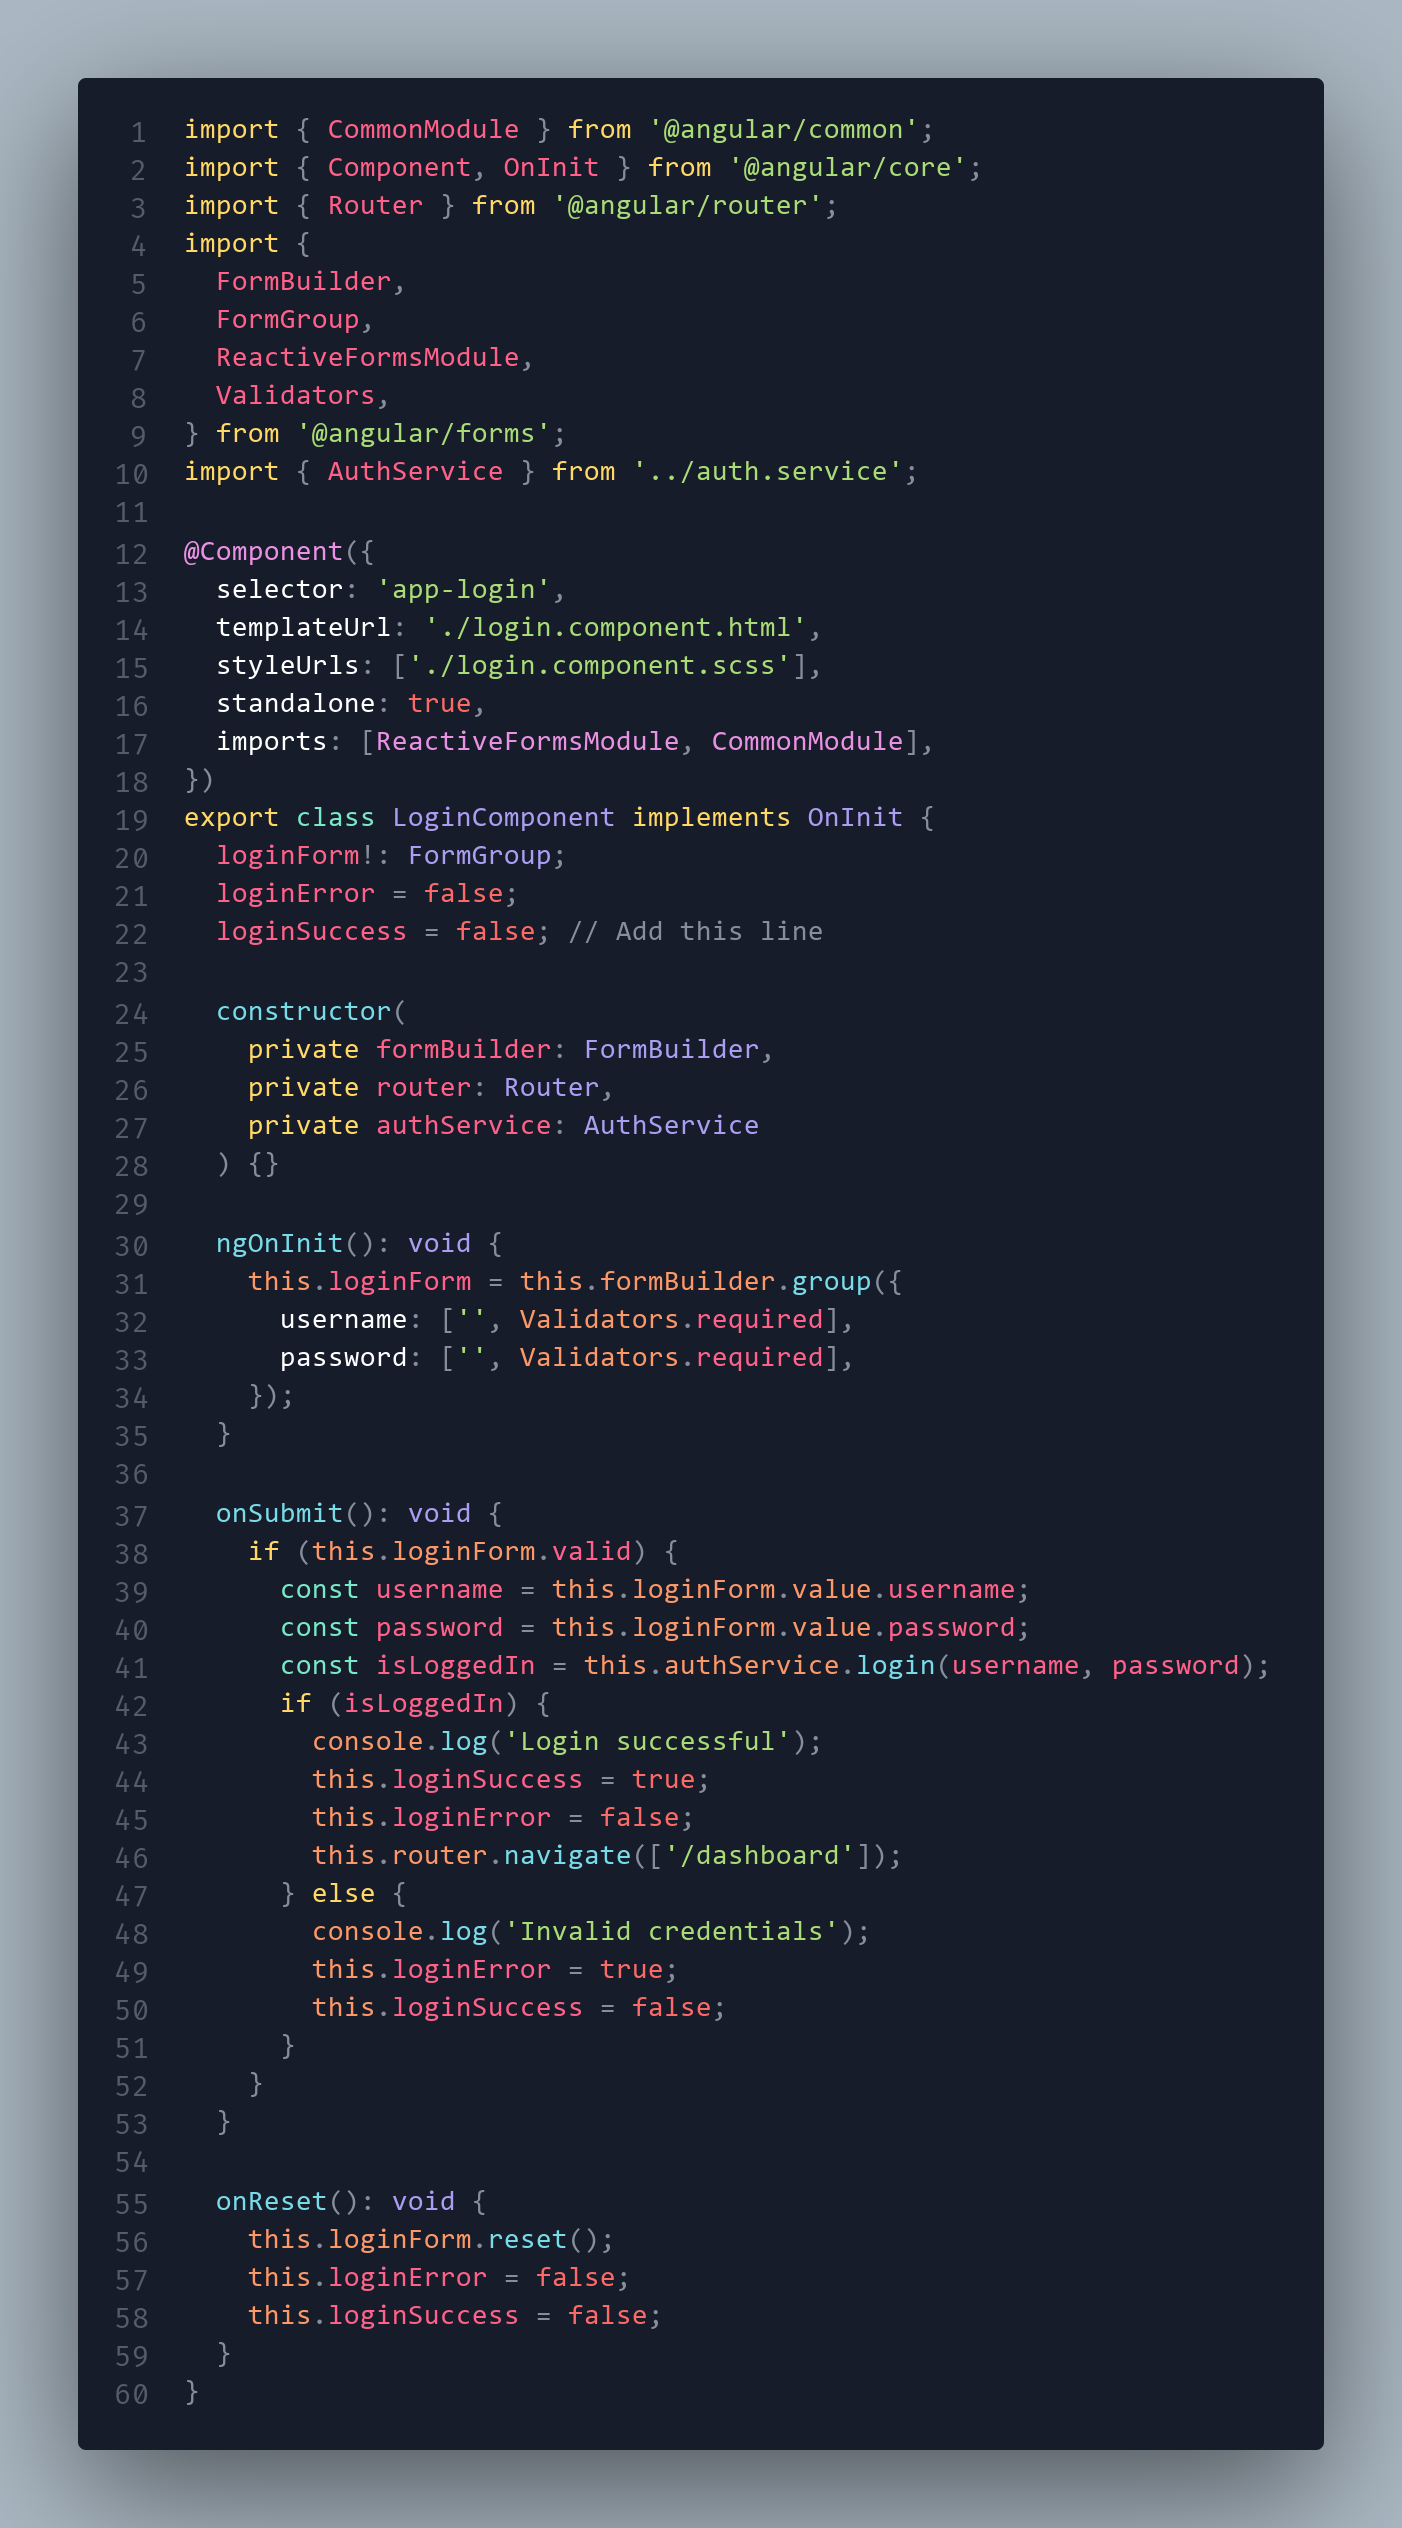
\includegraphics[height=0.75\textheight,keepaspectratio]{image-7.png}
  \caption{Zaimplementowany \texttt{login.component.ts}}
  \label{fig:image-7}
\end{figure}

%auth.service.ts
\subsubsection{\texttt{auth.service.ts}}
Komponent usługi odpowiedzialny za logowanie użytkownika.
\begin{figure}[H]
  \centering
  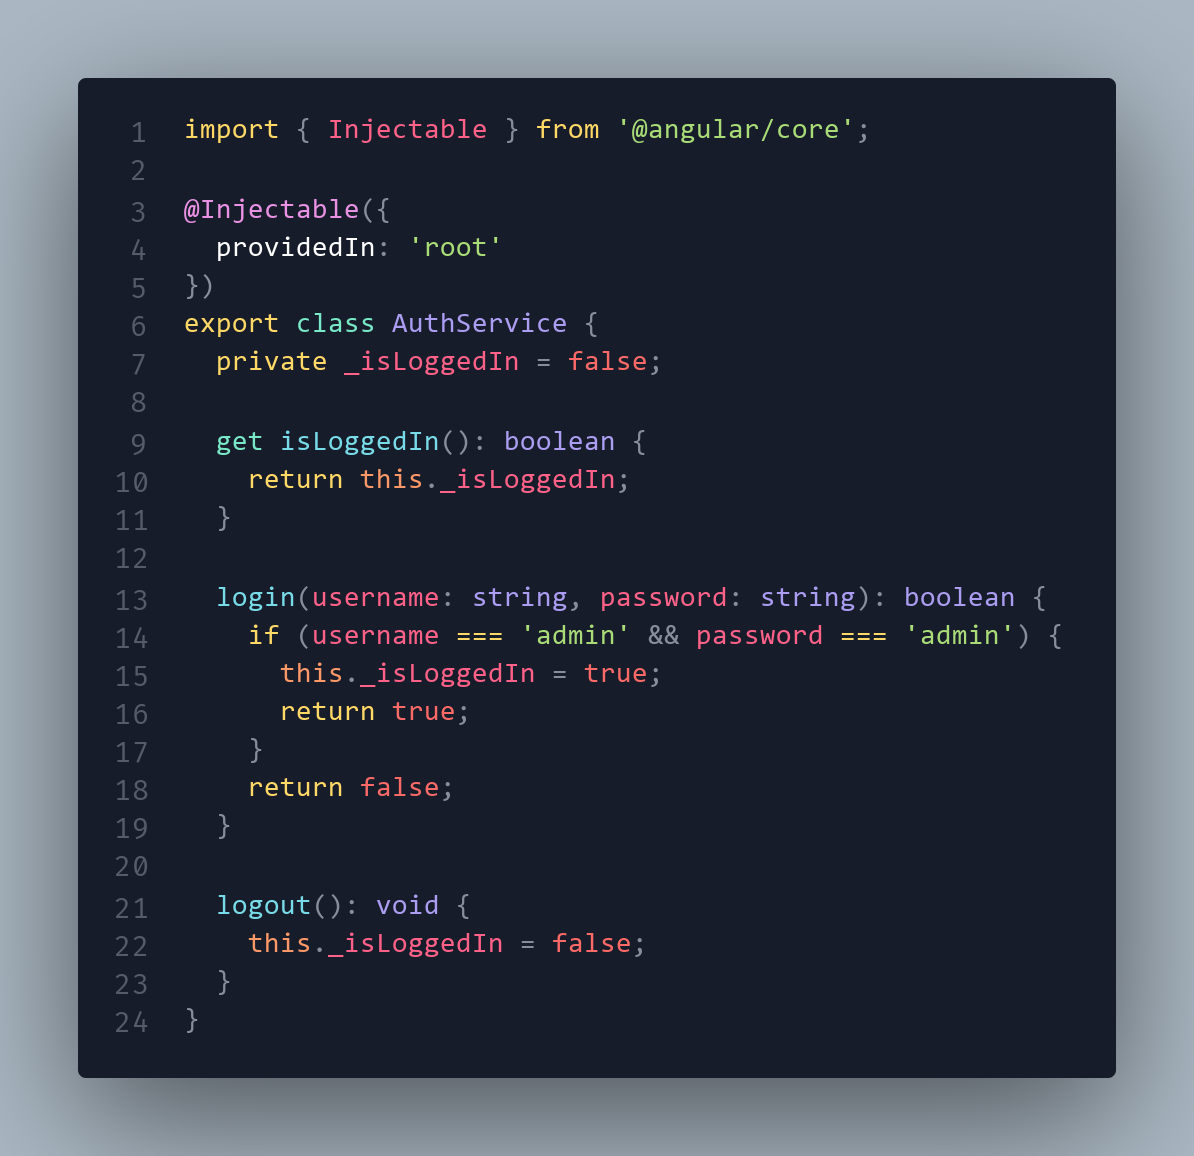
\includegraphics[width=\textwidth,height=\textheight,keepaspectratio]{image-8.png}
  \caption{Zaimplementowany \texttt{auth.service.ts}}
  \label{fig:image-8}
\end{figure}
% Image 4
\begin{figure}[H]
  \centering
  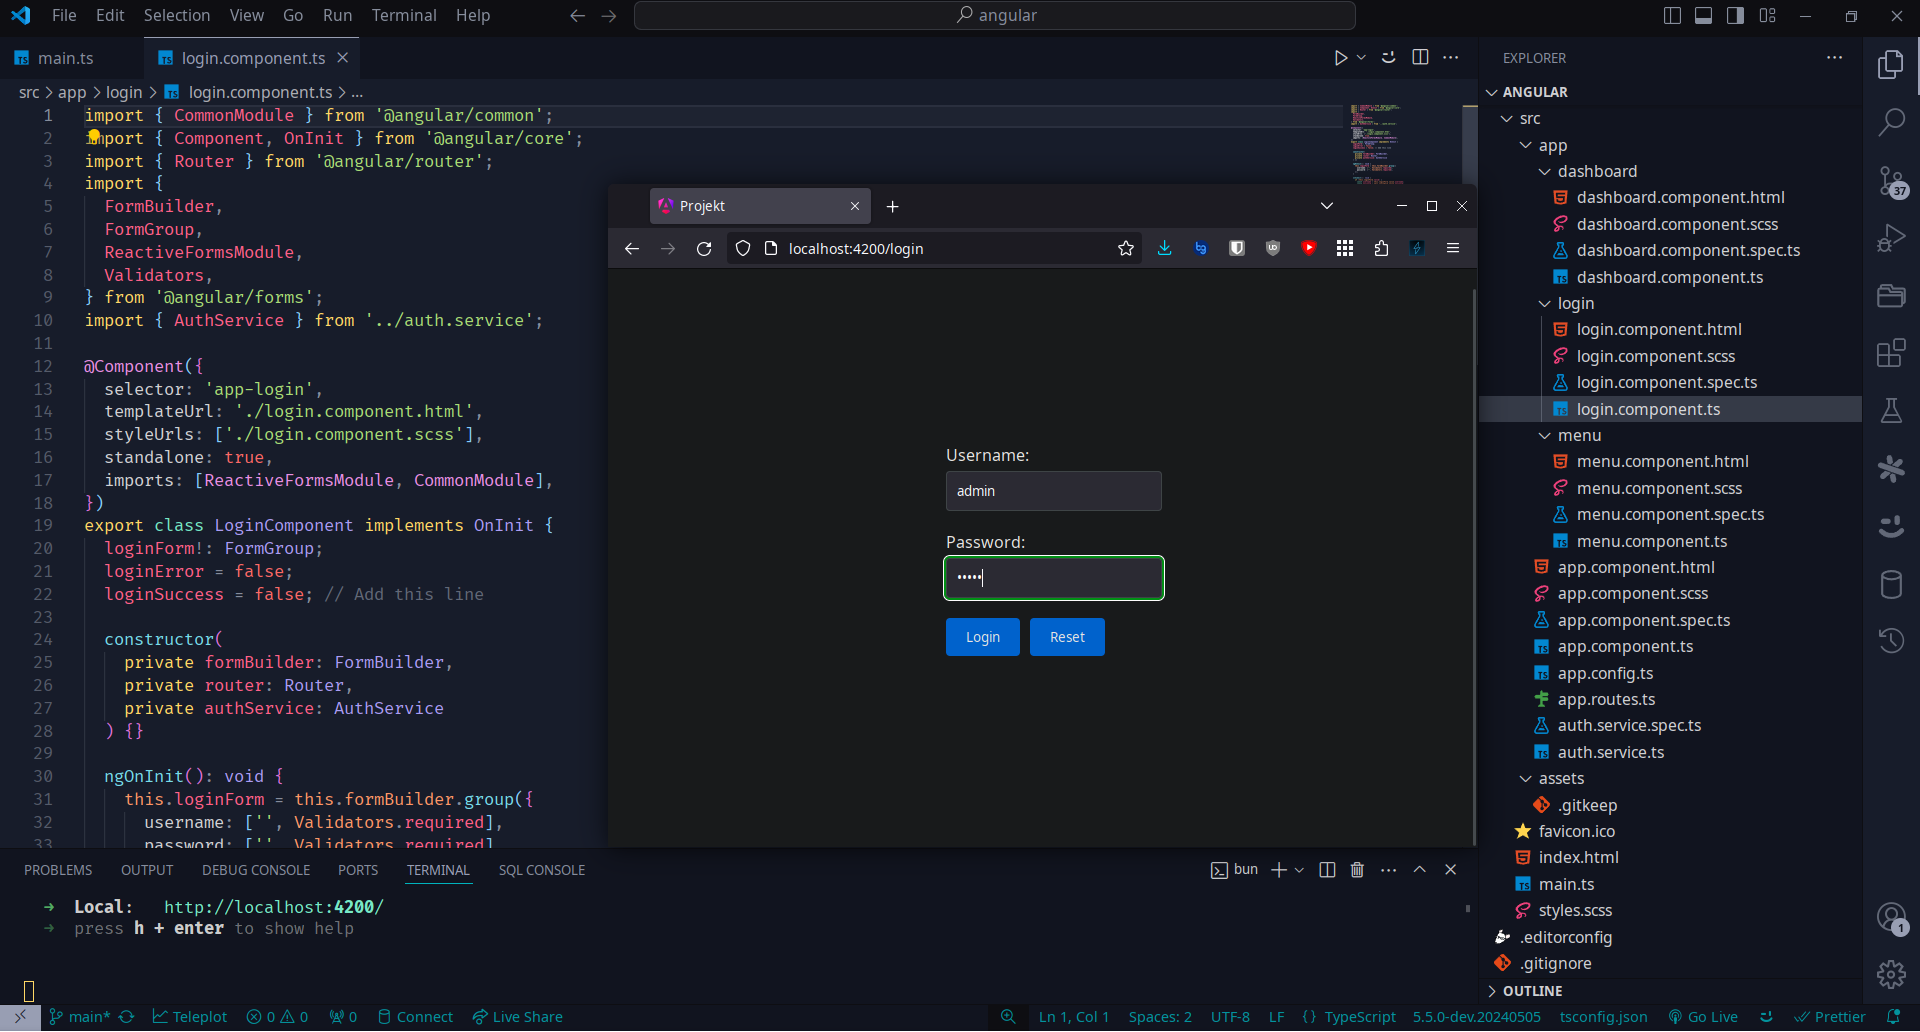
\includegraphics[width=1\textwidth]{image-3.png}
  \caption{Gotowy komponent logowania}
  \label{fig:image-3}
\end{figure}

\pagebreak

\subsection{Testy jednostkowe}
\begin{description}[leftmargin=.5em]
  \item{Napisanie testów dla komponentu logowanie, przy użyciu narzędzi takich jak \texttt{Jasmine} oraz \texttt{Karma}}. Wzorowanie się na załączonym przez prowadzącego kodzie testu podczas pisania własnej implementacji.
\end{description}
% Image 4
\begin{figure}[H]
  \centering
  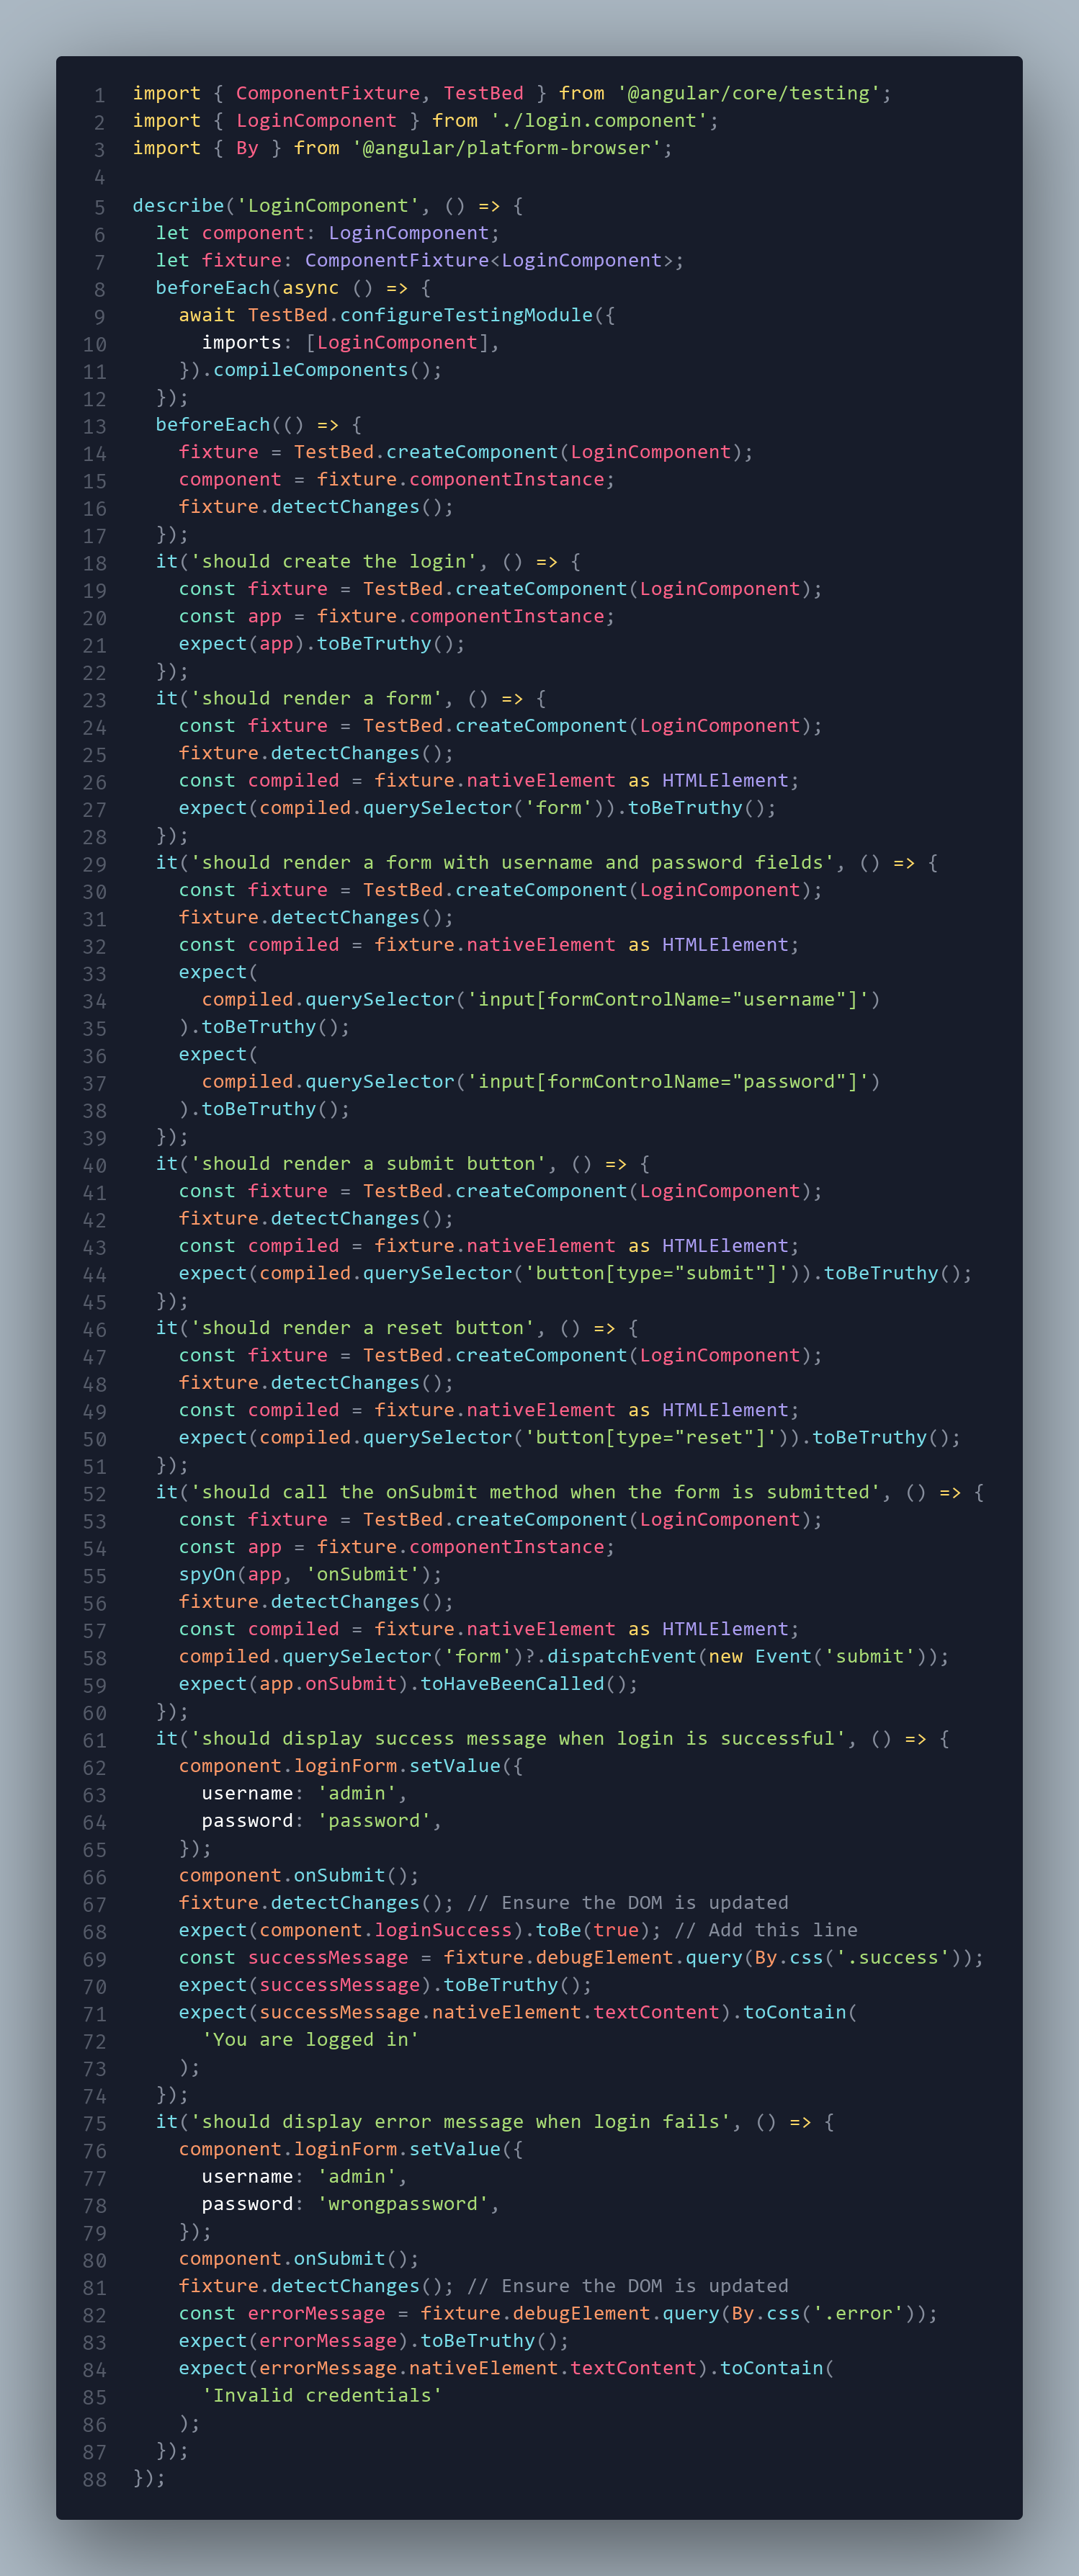
\includegraphics[height=0.79\textheight,keepaspectratio]{image-9.png}
  \caption{Własna implementacja funkcji testujących komponent logowania}
  \label{fig:image-9}
\end{figure}
\begin{figure}[H]
  \centering
  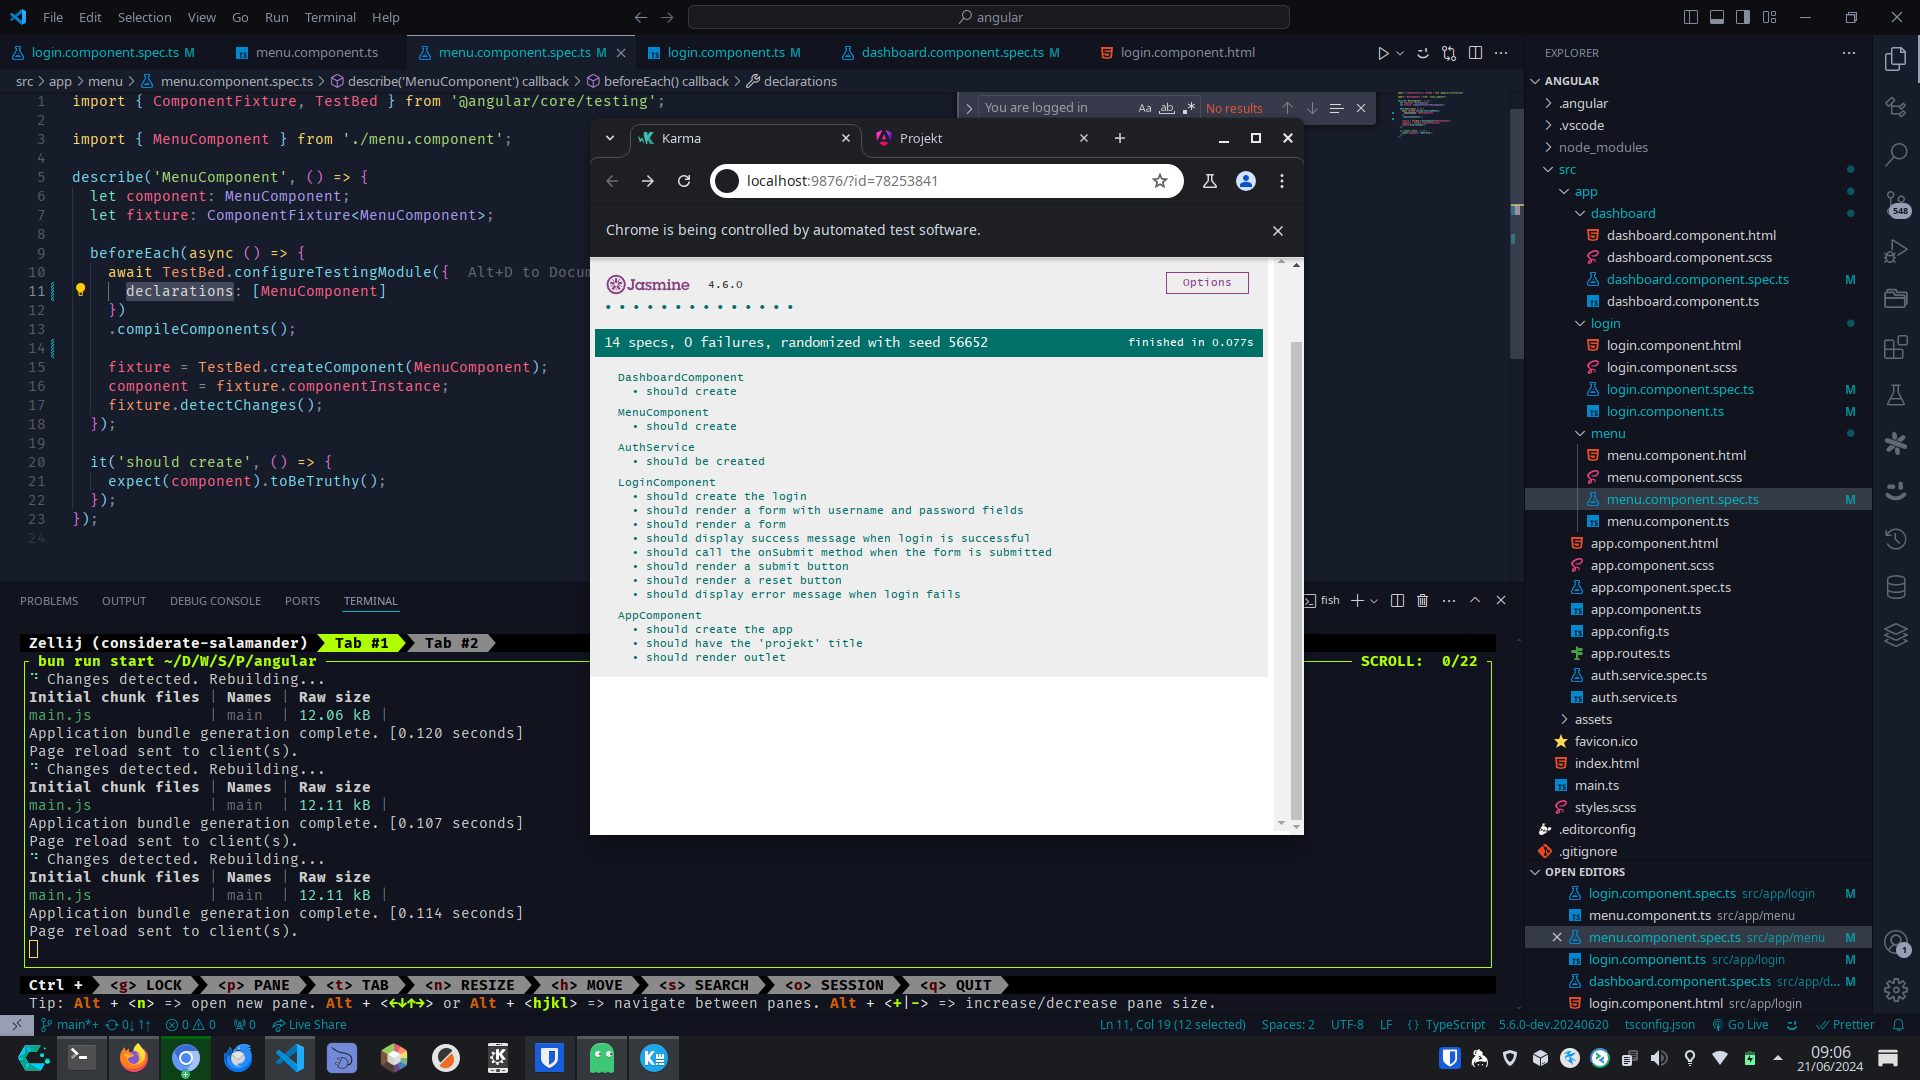
\includegraphics[width=1\textwidth,keepaspectratio]{image-10.png}
  \caption{Wyniki testowania}
  \label{fig:image-10}
\end{figure}

\pagebreak

\subsection{Dodawanie dashboardu}
\begin{itemize}[leftmargin=.5em]
  \item{Utworzenie komponentu \texttt{dashboard}}
  \item{Utworzenie routingu}
  \item{Utworzenie komponentu \texttt{menu}}
  \item{Wykorzystanie wcześniej utworzonej usługi \texttt{auth}}
  \item{Utworzenie testów dla komponentu \texttt{dashboard}}
\end{itemize}

\subsubsection{Utworzenie komponentu \texttt{dashboard}}
\begin{figure}[H]
  \centering
  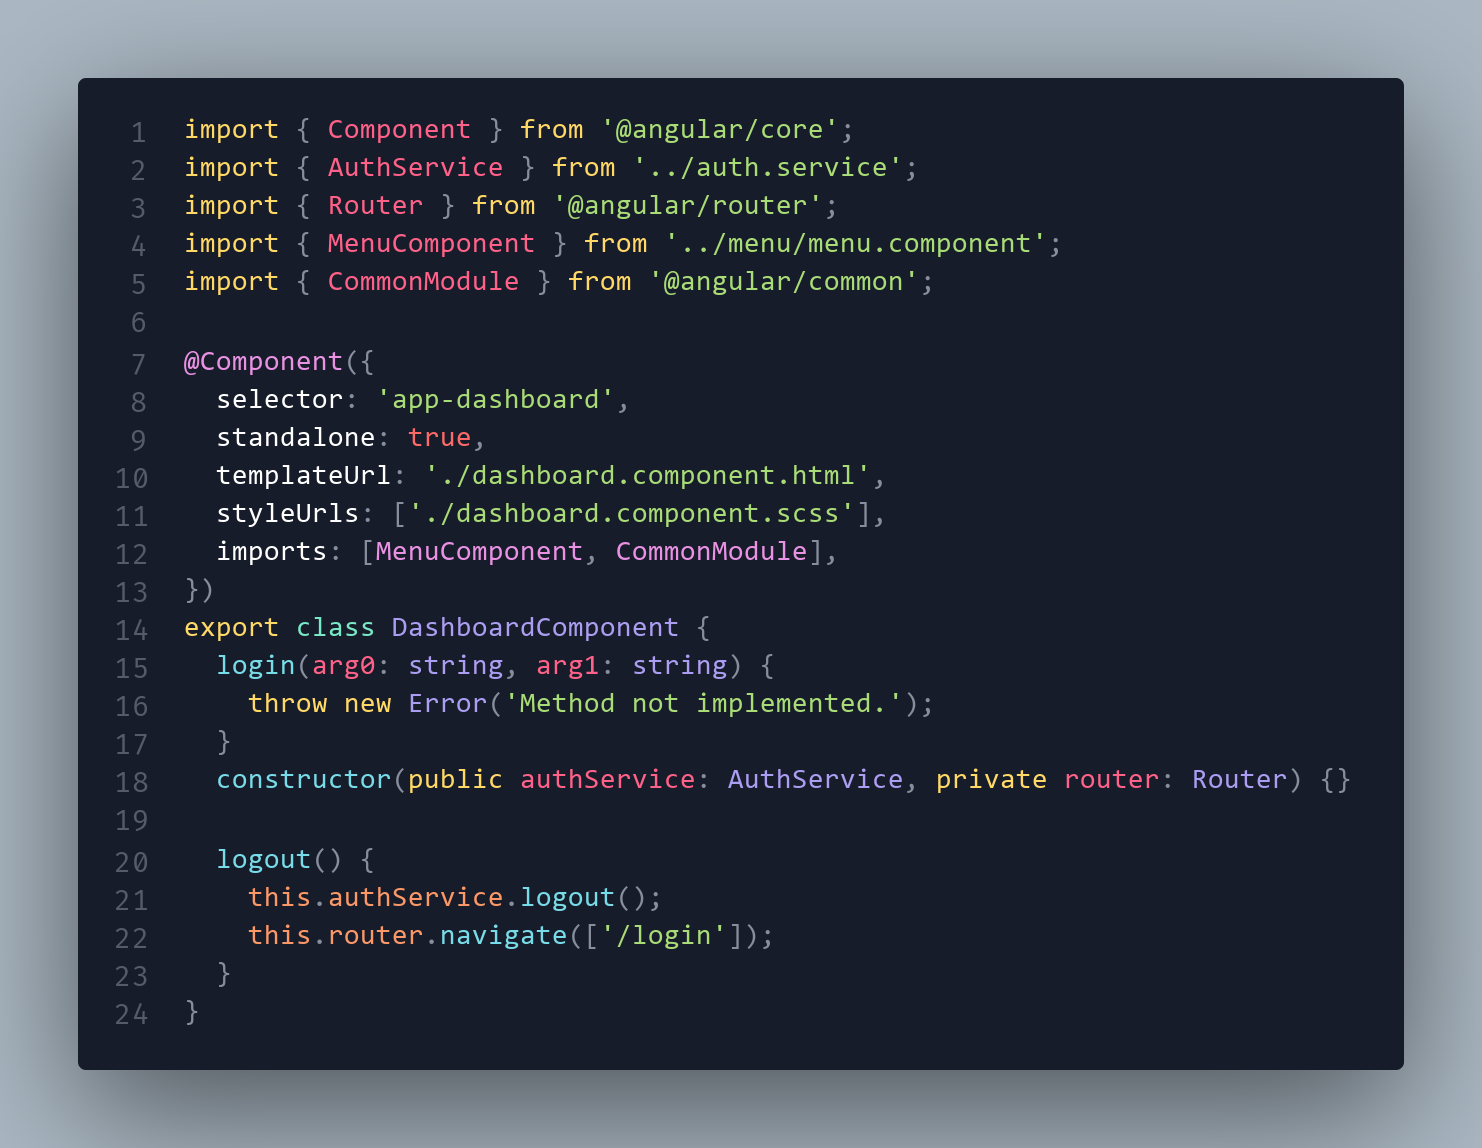
\includegraphics[width=1\textwidth,keepaspectratio]{image-11.png}
  \caption{Implementacja \texttt{dashboard.component.ts}}
  \label{fig:image-11}
\end{figure}
\begin{figure}[H]
  \centering
  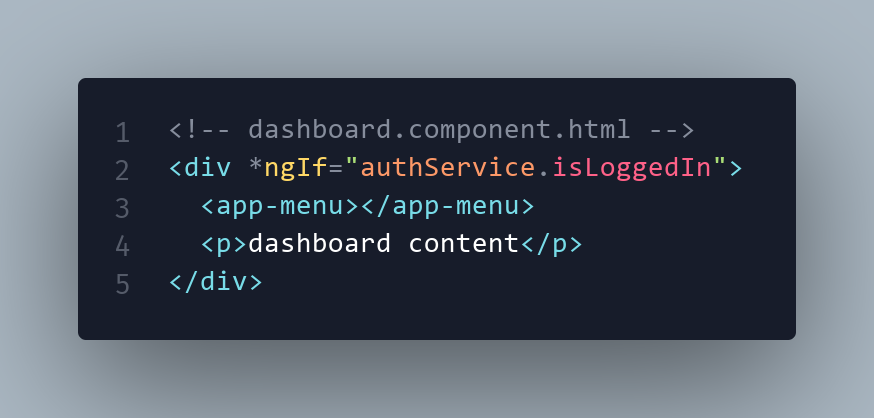
\includegraphics[width=1\textwidth,keepaspectratio]{image-12.png}
  \caption{Implementacja \texttt{dashboard.component.html}}
  \label{fig:image-12}
\end{figure}

\subsubsection{Utworzenie routingu}
\begin{figure}[H]
  \centering
  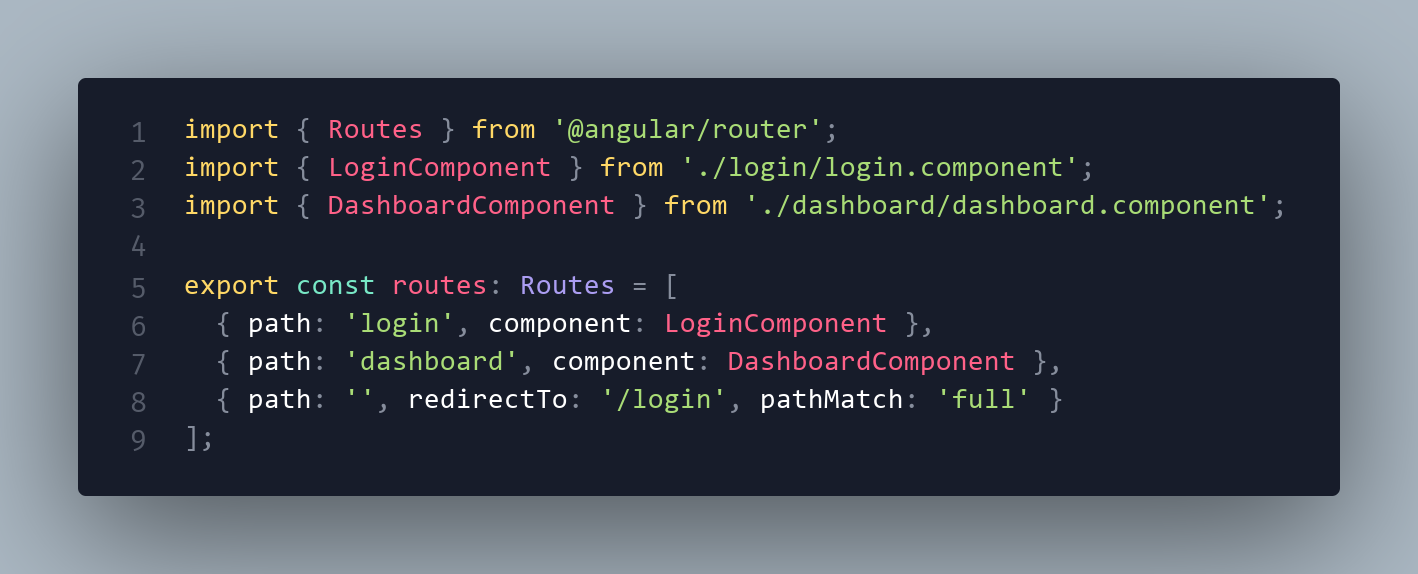
\includegraphics[width=1\textwidth,keepaspectratio]{image-14.png}
  \caption{Implementacja \texttt{app.routes.ts}}
  \label{fig:image-14}
\end{figure}

\pagebreak

\subsubsection{Utworzenie komponentu \texttt{menu}}
Wykorzystanie do tego przygotowanej wcześniej usługi \texttt{auth}.
\begin{figure}[H]
  \centering
  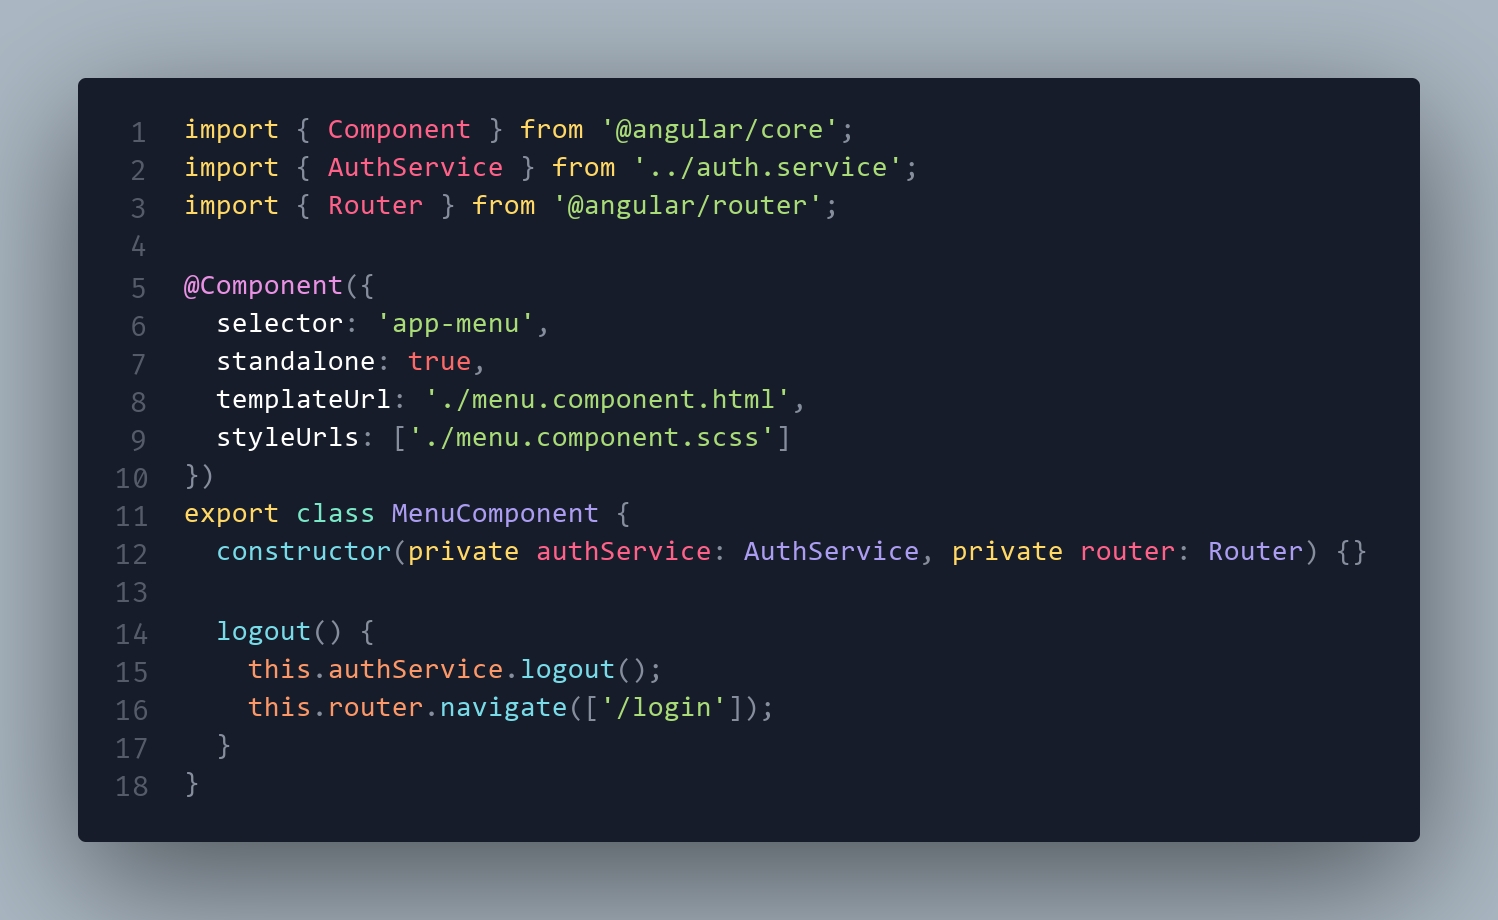
\includegraphics[width=0.95\textwidth,keepaspectratio]{image-15.png}
  \caption{Implementacja \texttt{menu.component.ts}}
  \label{fig:image-15}
\end{figure}
\begin{figure}[H]
  \centering
  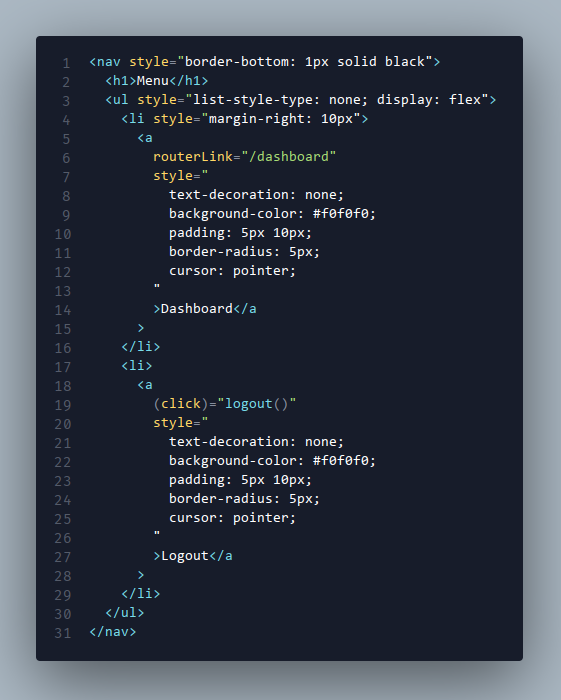
\includegraphics[width=1\textwidth,keepaspectratio]{image-16.png}
  \caption{Implementacja \texttt{menu.component.html}}
  \label{fig:image-16}
\end{figure}
\begin{figure}[H]
  \centering
  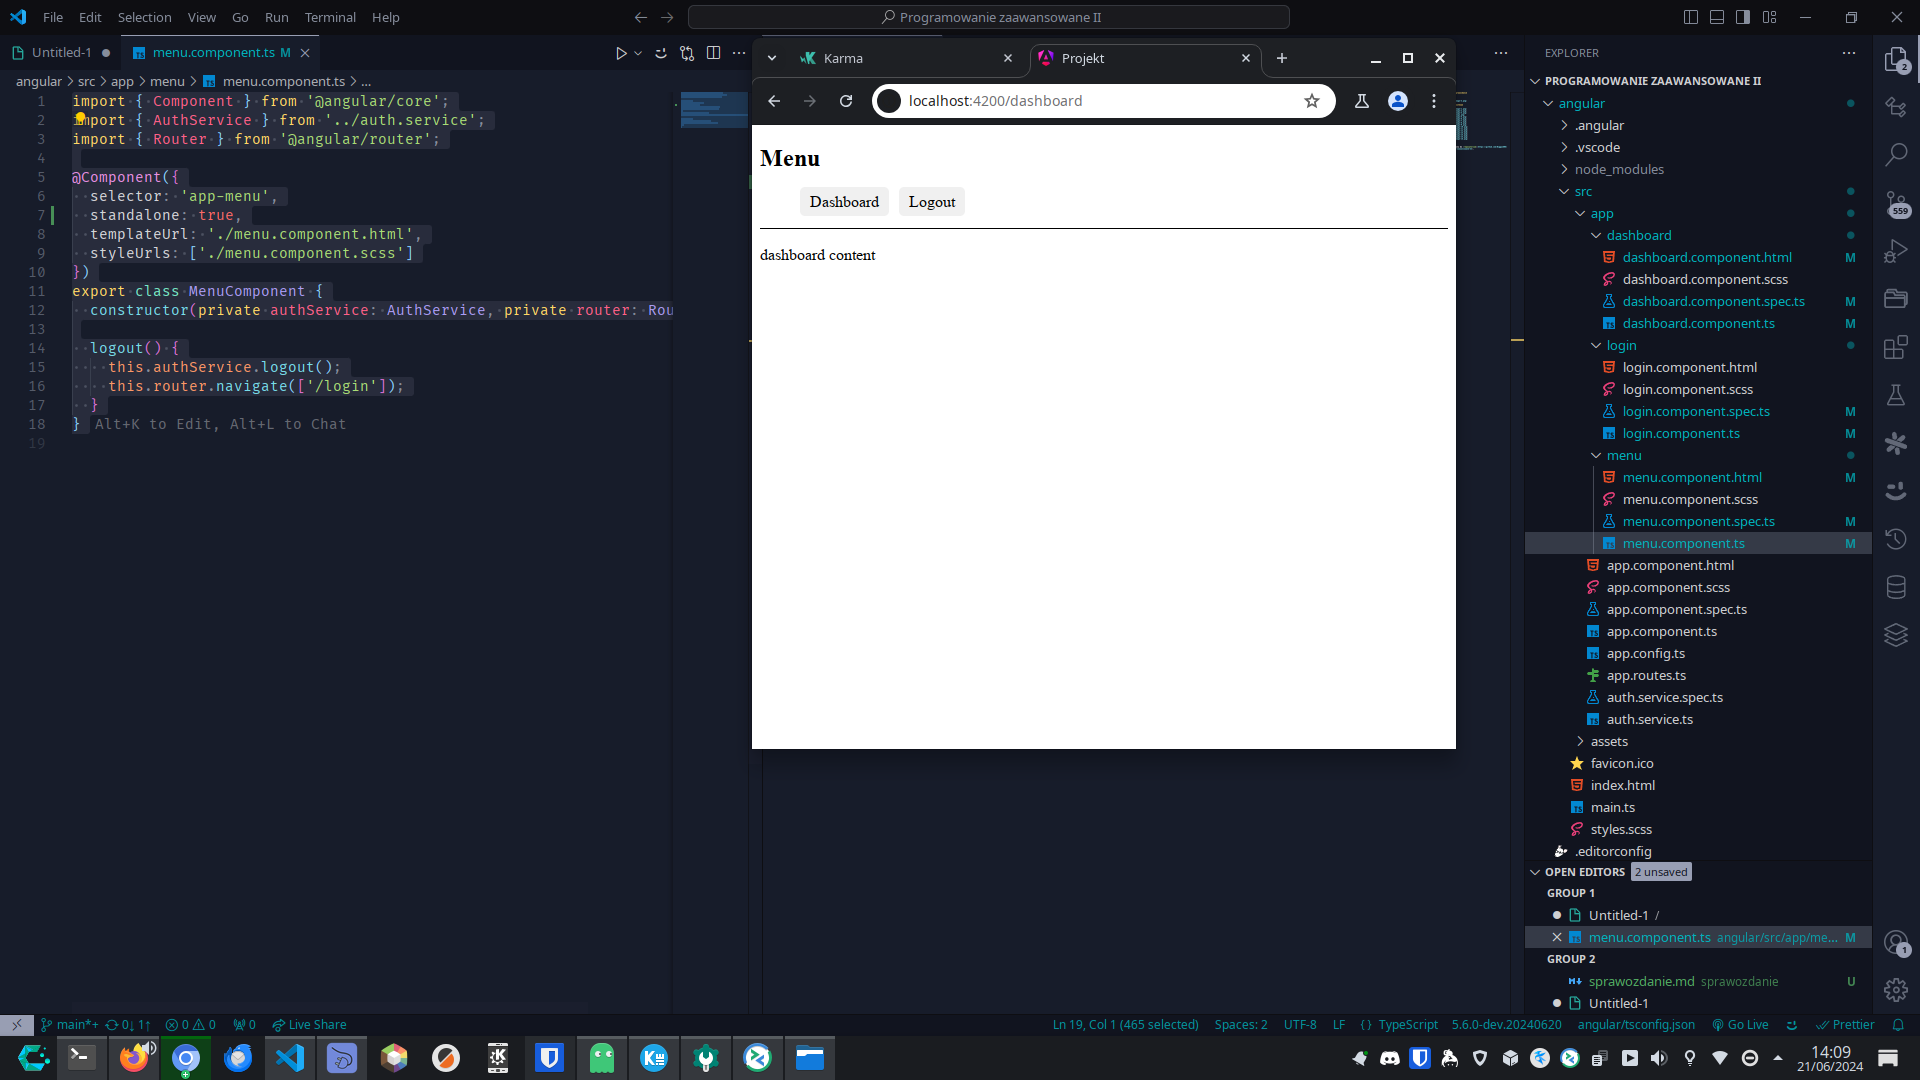
\includegraphics[width=1\textwidth,keepaspectratio]{image-17.png} \caption{Prezentacja działających komponentów}
  \label{fig:image-17}
\end{figure}
\vspace*{\fill}

\subsubsection{Utworzenie testów dla komponentu \texttt{dashboard}}
Wykorzystanie dostarczonych przez prowadzącego propozycji kodu w opracowaniu własnej implementacji.
\begin{figure}[H]
  \centering
  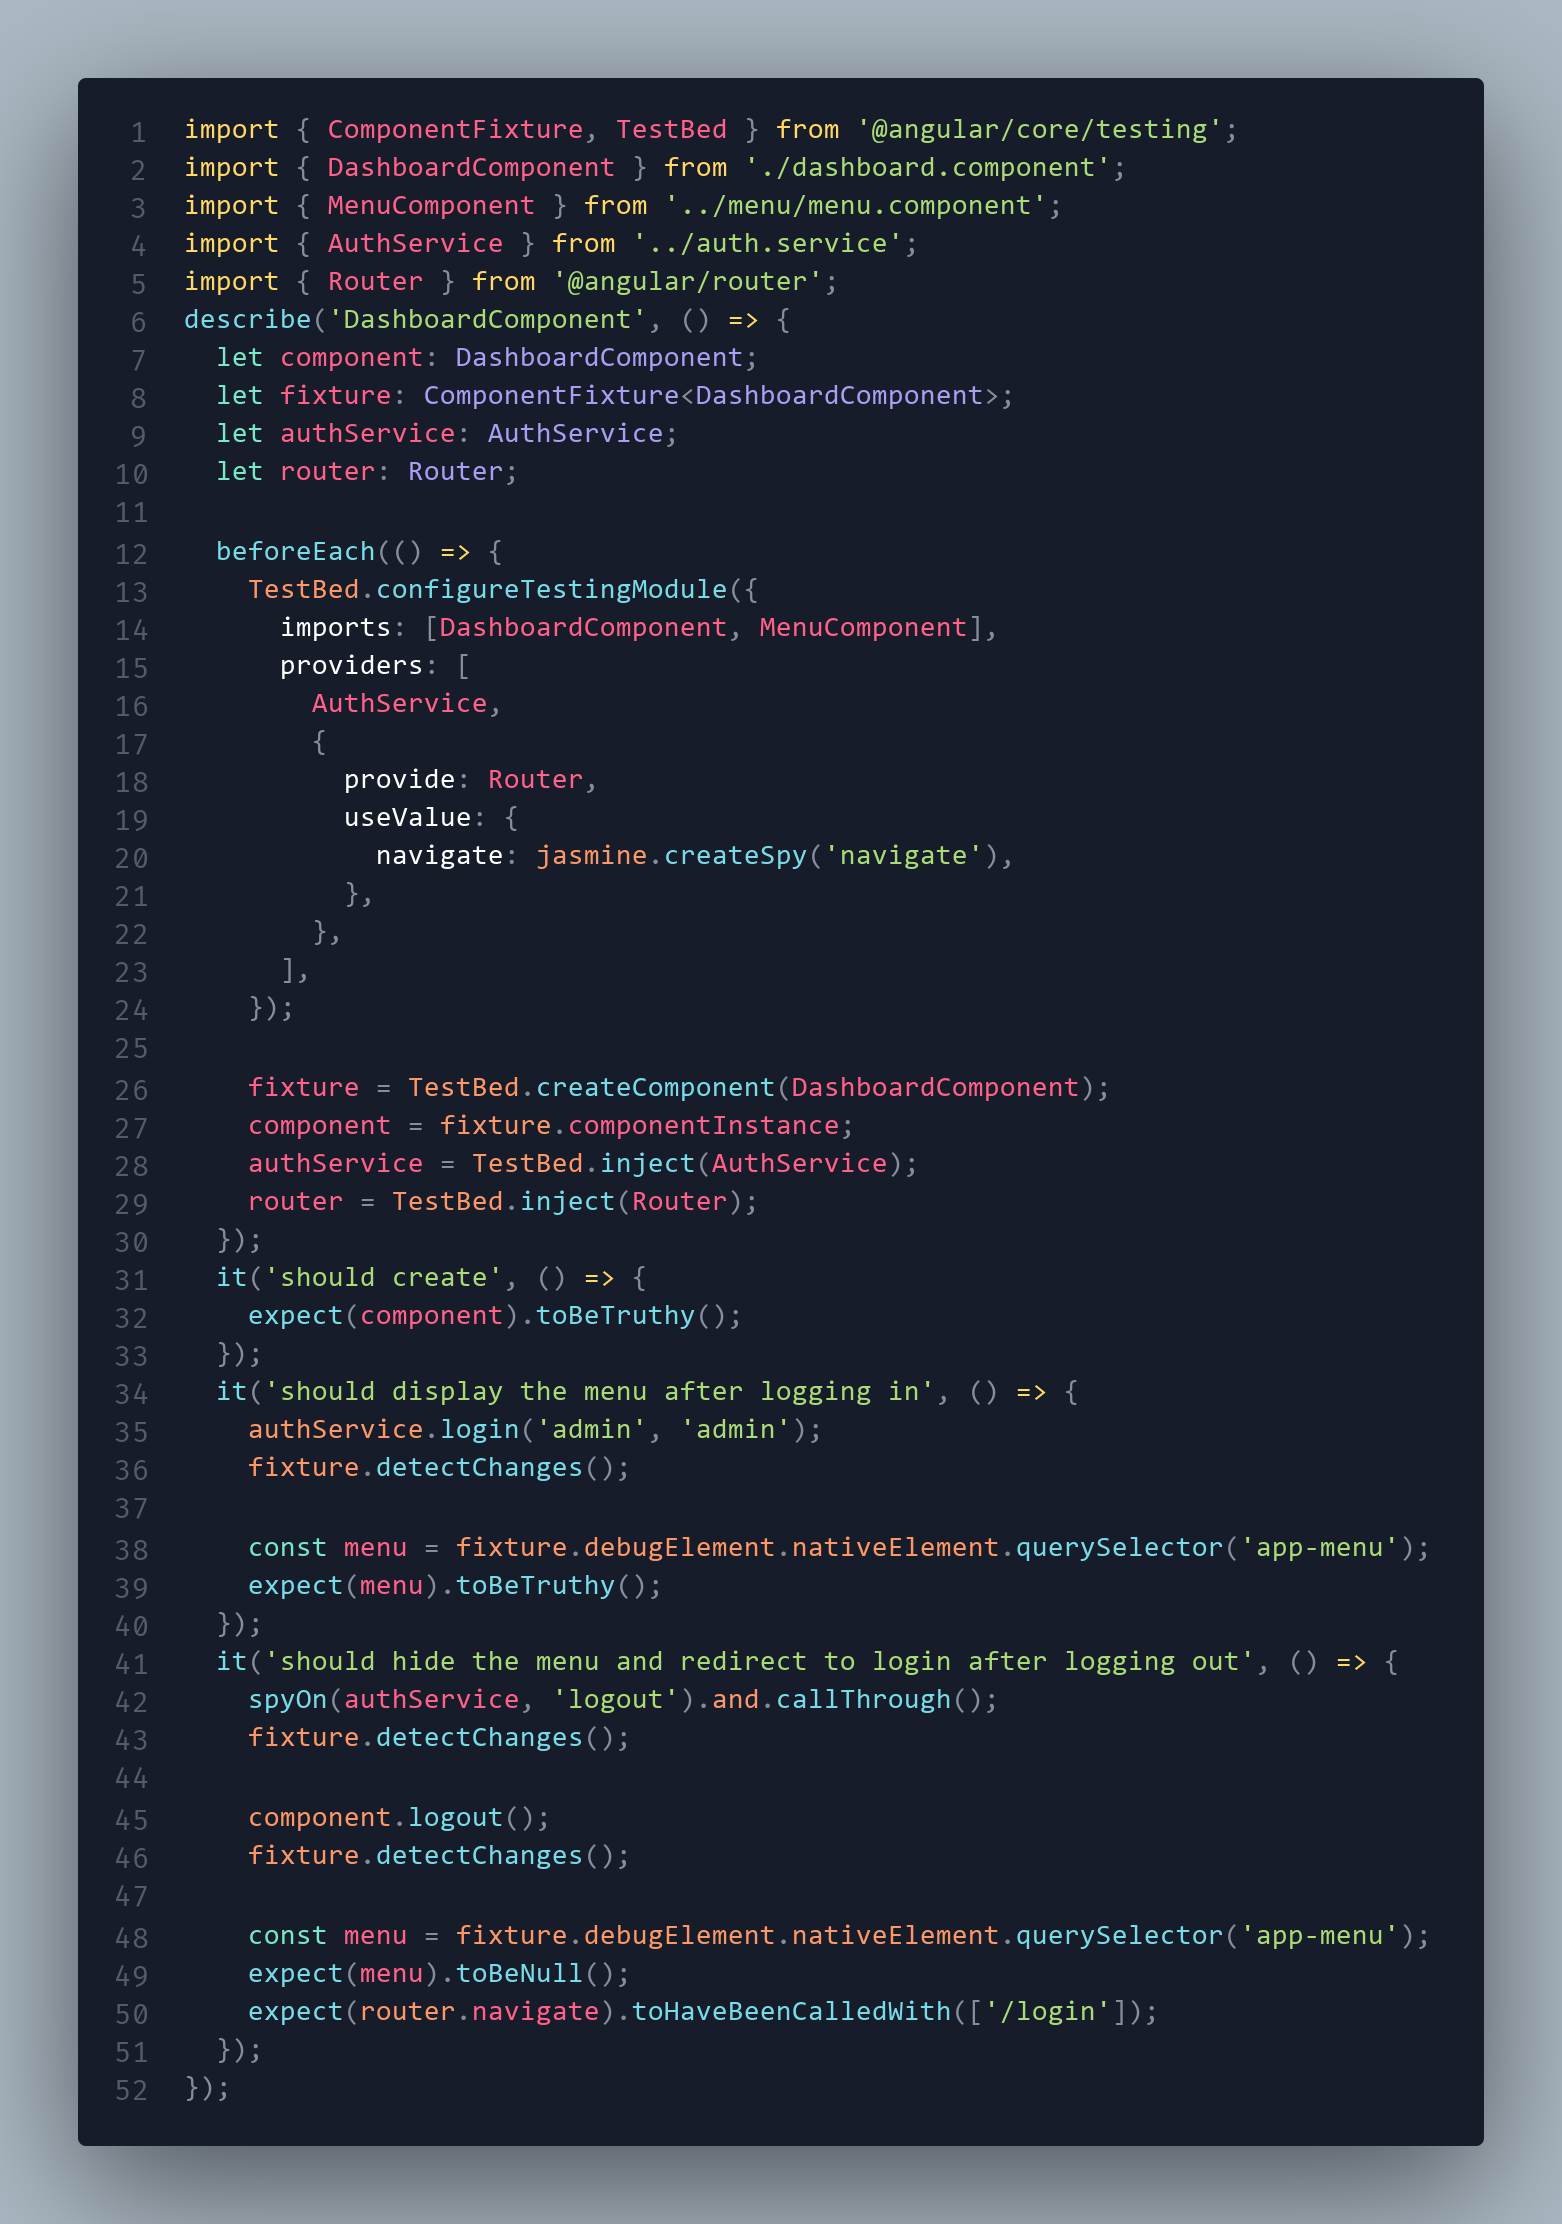
\includegraphics[width=0.82\textwidth,keepaspectratio]{image-13.png}
  \caption{Implementacja \texttt{dashboard.component.spec.ts}}
  \label{fig:image-13}
\end{figure}
Poniższe zdjęcie przedstawia różnice pomiędzy proponowaną implementacją testu komponentu dashboard.component.spec.ts a ostateczną wersją. Problematyczny okazał się ostatni test, w którym sprawdzano, czy komponent nie jest renderowany. W proponowanym podejściu test ten nie przechodził.
\begin{figure}[H]
  \centering
  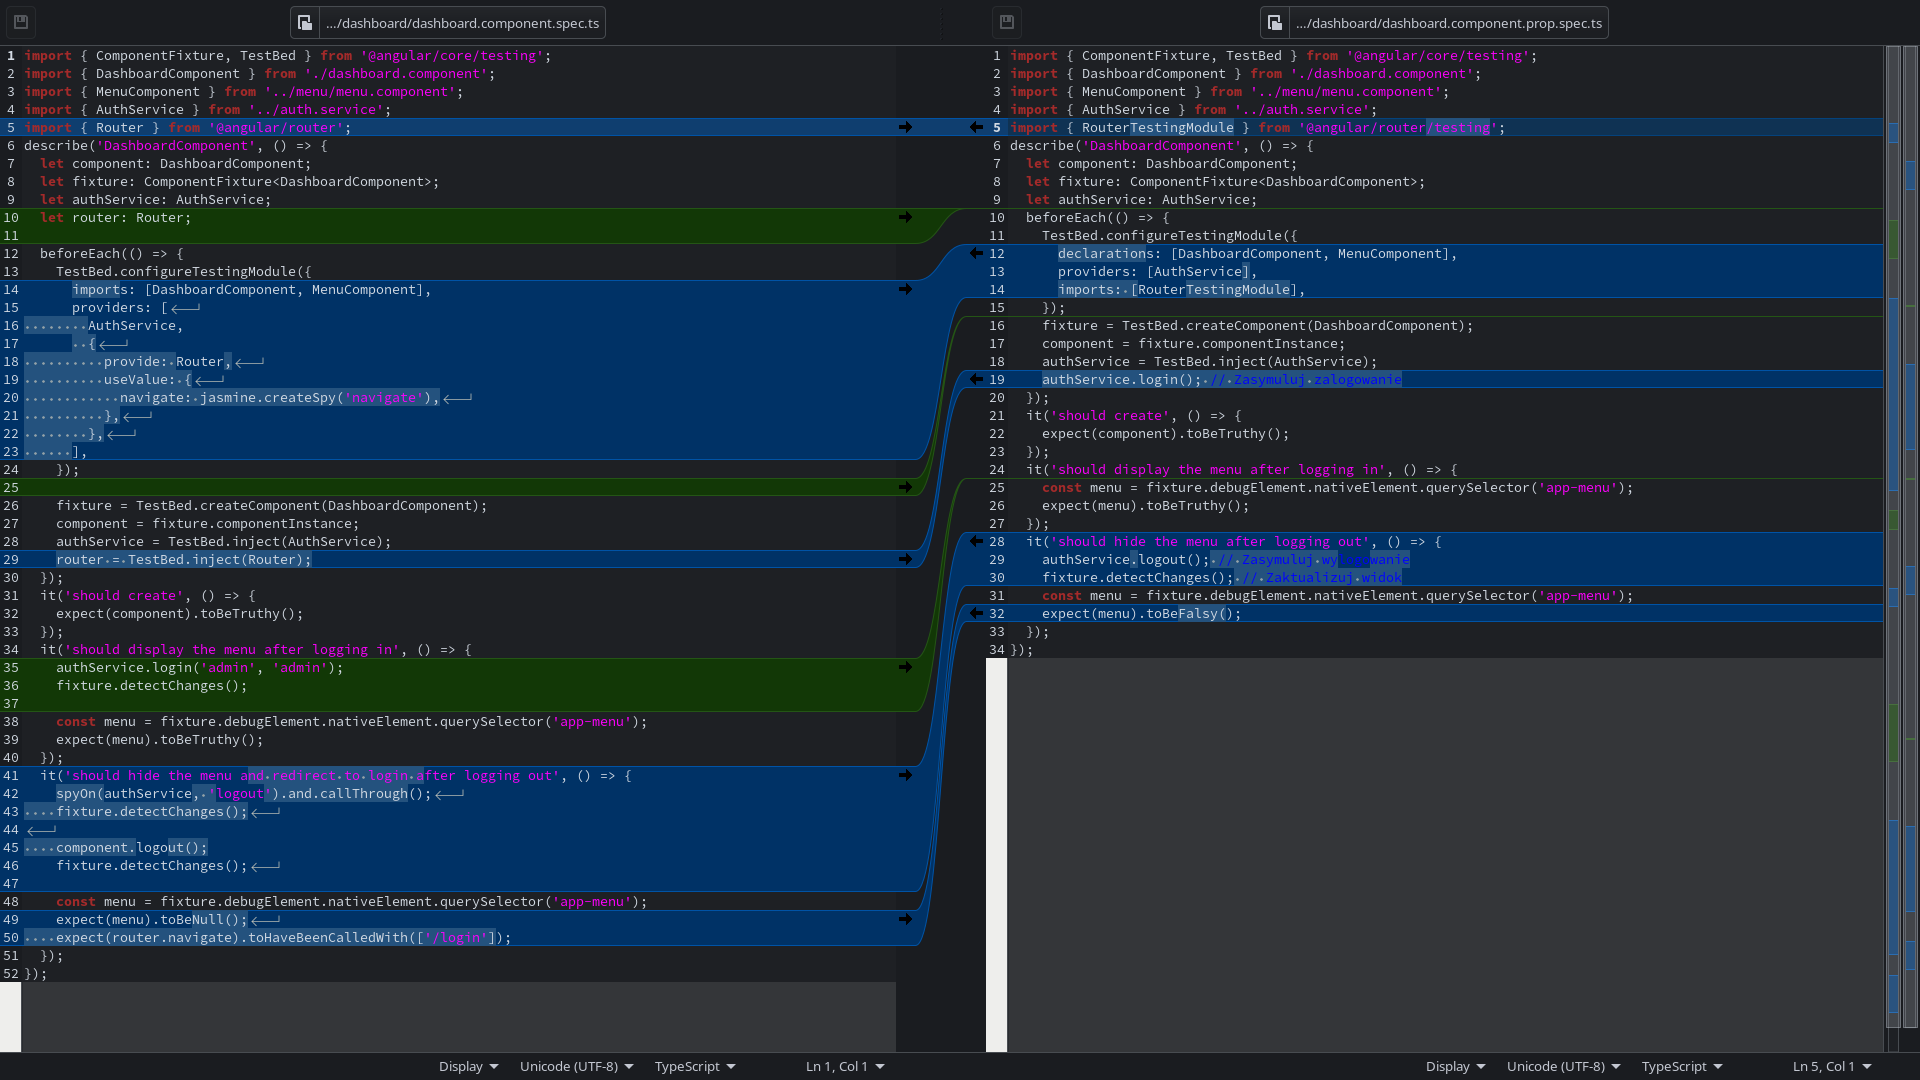
\includegraphics[width=1\textwidth,keepaspectratio]{image-19.png}
  \caption{Porównanie konfiguracji testów komponentu \texttt{dashboard.component.spec.ts}}
  \label{fig:image-19}
\end{figure}
\begin{figure}[H]
  \centering
  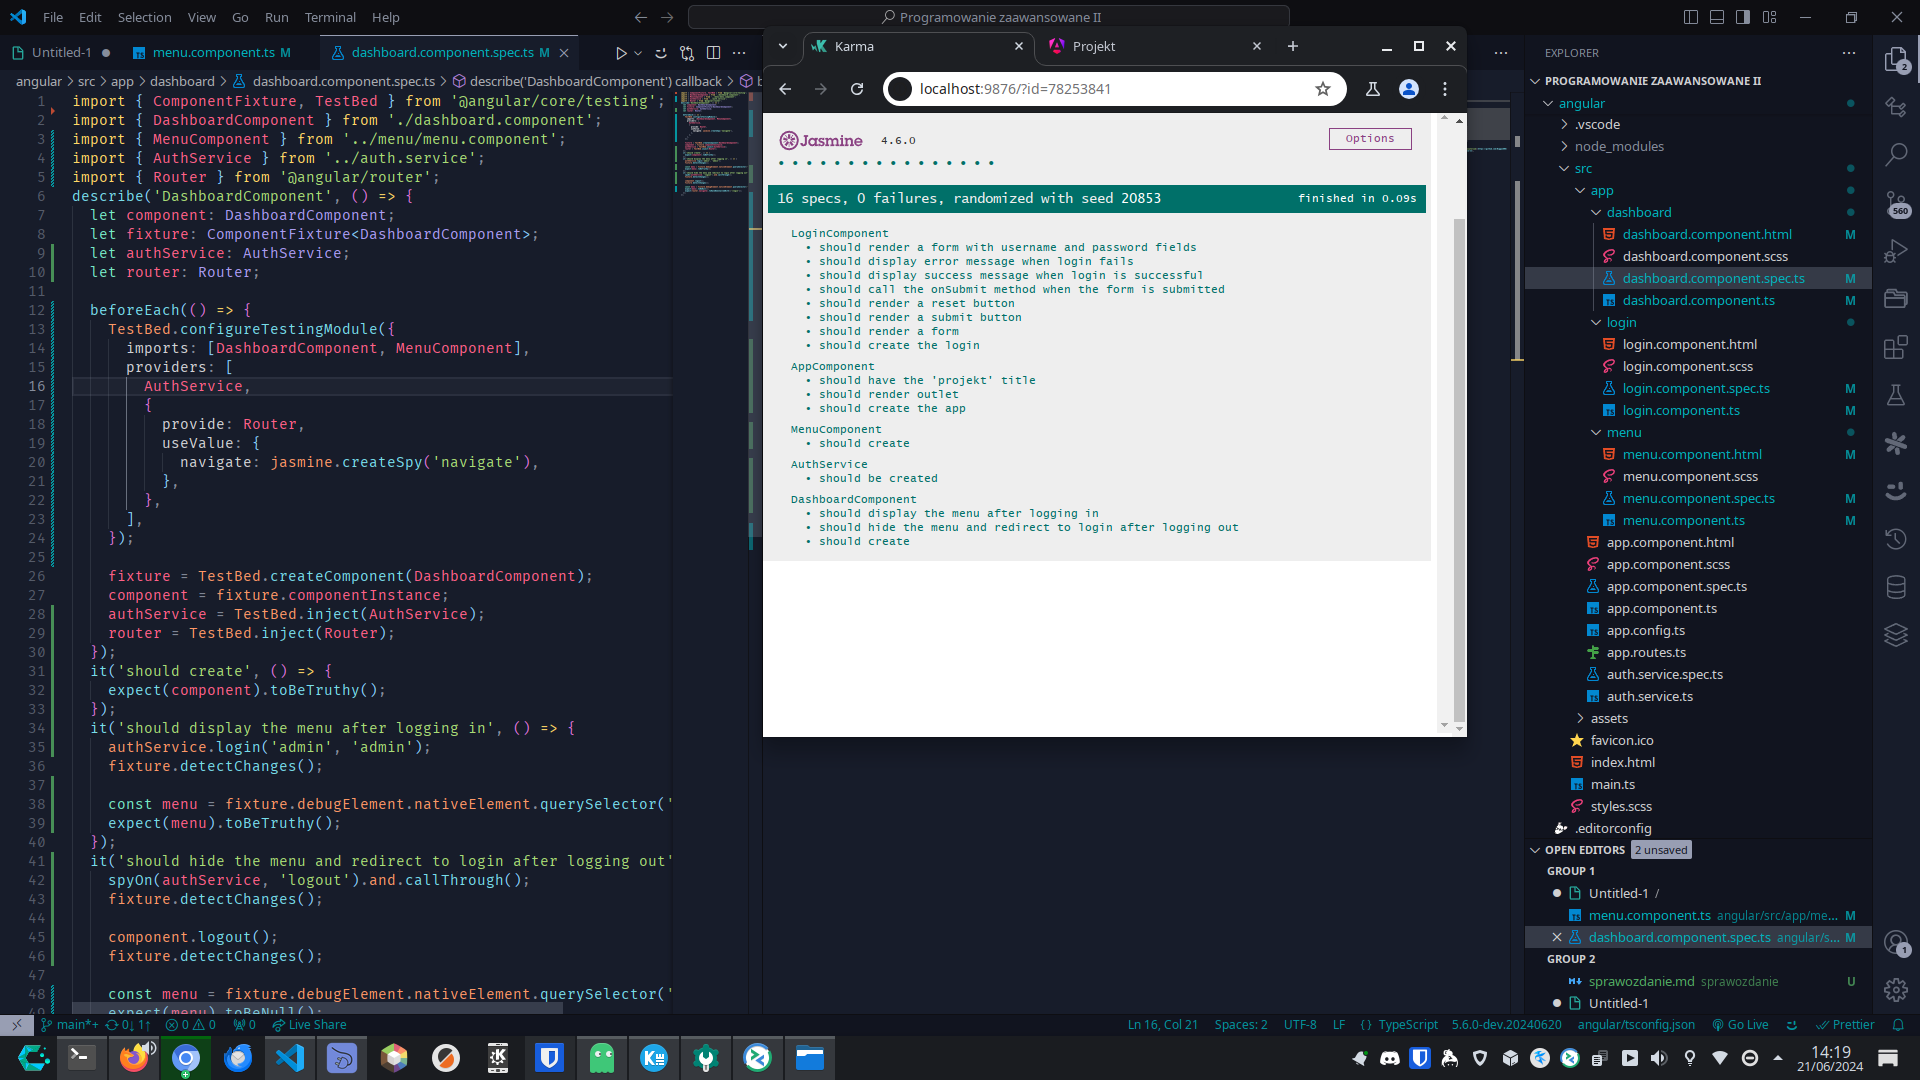
\includegraphics[width=0.82\textwidth,keepaspectratio]{image-18.png}
  \caption{Pokrycie testów \texttt{Karma}}
  \label{fig:image-18}
\end{figure}
\pagebreak
\section{Tworzenie testów automatycznych systemu w podejściu TDD}
\begin{figure}[H]
  \centering
  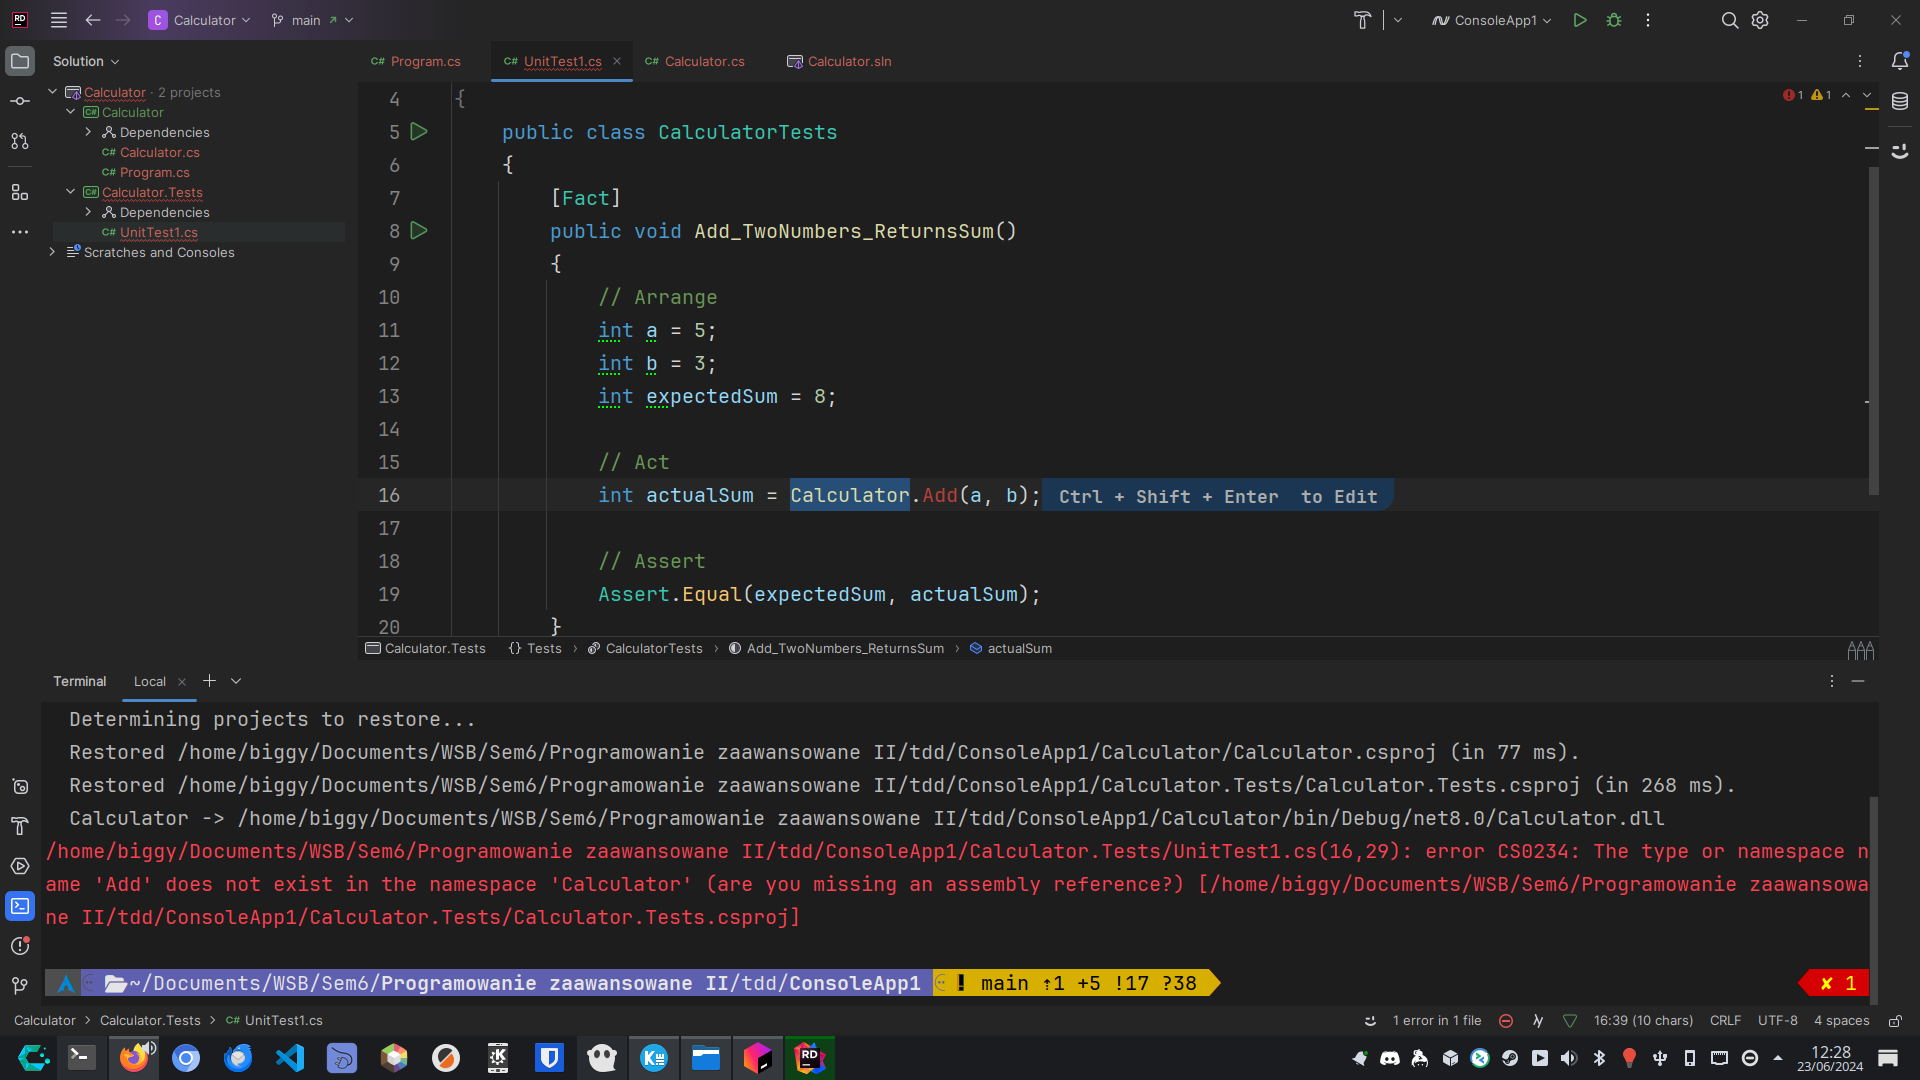
\includegraphics[width=0.85\textwidth,keepaspectratio]{image-20.png}
  \caption{Fail testu, brak funkcjonalności w testowanej klasie}
  \label{fig:image-20}
\end{figure}
\begin{figure}[H]
  \centering
  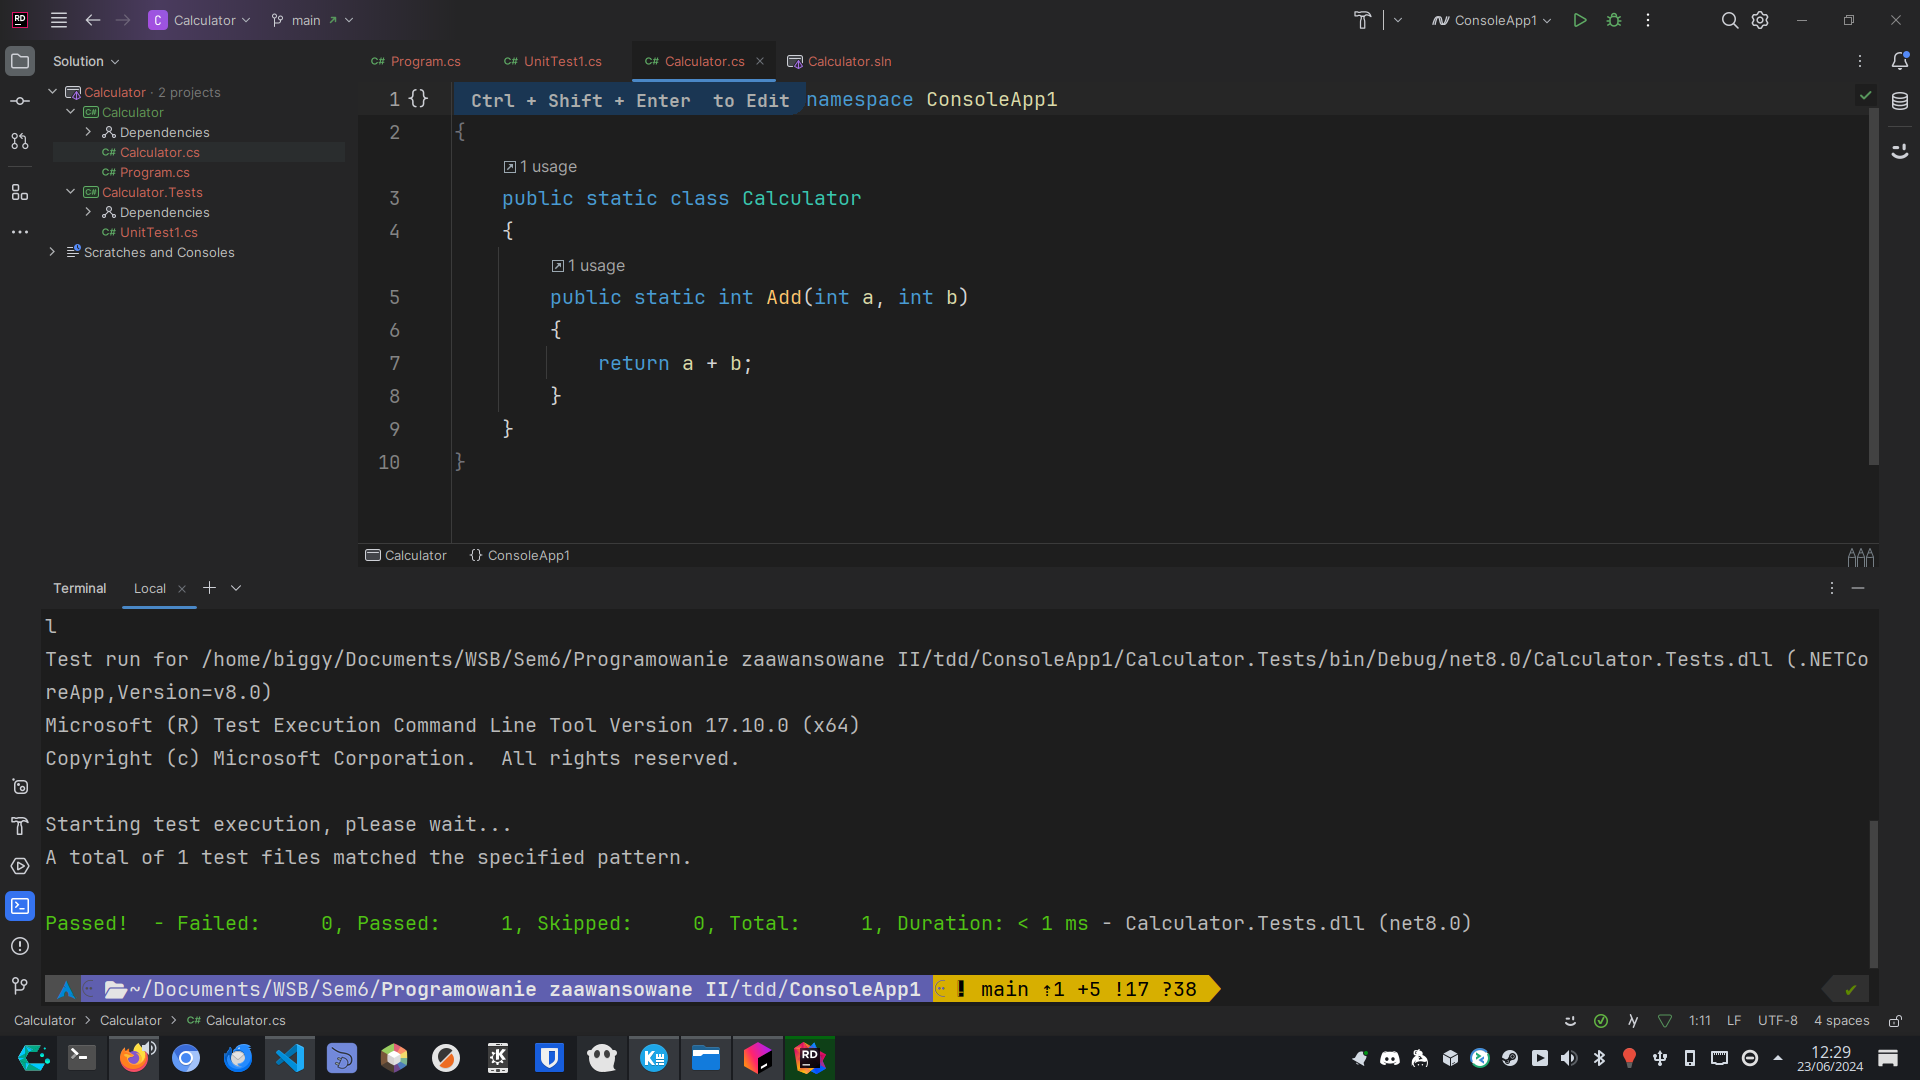
\includegraphics[width=0.85\textwidth,keepaspectratio]{image-21.png}
  \caption{Dodanie oczekiwanej metody do tesowanej klasy}
  \label{fig:image-21}
\end{figure}
Przedstawiony kod został napisany na tyle prosto i przejrzyście że nie wymaga refaktoryzacji.
\begin{minted}{csharp}
using Xunit;

namespace Calculator.Tests {
    public class CalculatorTests {
        [Fact]
        public void Add_TwoNumbers_ReturnsSum() {
            // Arrange
            int a = 5;
            int b = 3;
            int expectedSum = 8;
            // Act
            int actualSum = Calculator.Add(a, b);
            // Assert
            Assert.Equal(expectedSum, actualSum);
        }
    }
}
\end{minted}
\begin{minted}{csharp}
namespace Calculator {
    public static class Calculator {
        public static int Add(int a, int b) {
            return a + b;
        }
    }
}
\end{minted}
\pagebreak
\section{Testowania testów automatycznych systemu w podejściu BDD}
\begin{description}
  \item{Ze względu na brak kompatybilności \texttt{SpecFlow} z Visual Studio 2022, zastosowano alternatywne narzędzie \texttt{Reqnroll}. Proces użytkowania \texttt{Reqnroll} okazał się bardzo zbliżony do \texttt{SpecFlow}. Mimo że problem ten znacząco utrudnił realizację zadania, ostatecznie udało się je pomyślnie ukończyć.}
        \textit{Na potrzeby zadania użyłem środowiska Windows'owego}

\end{description}
\begin{figure}[H]
  \centering
  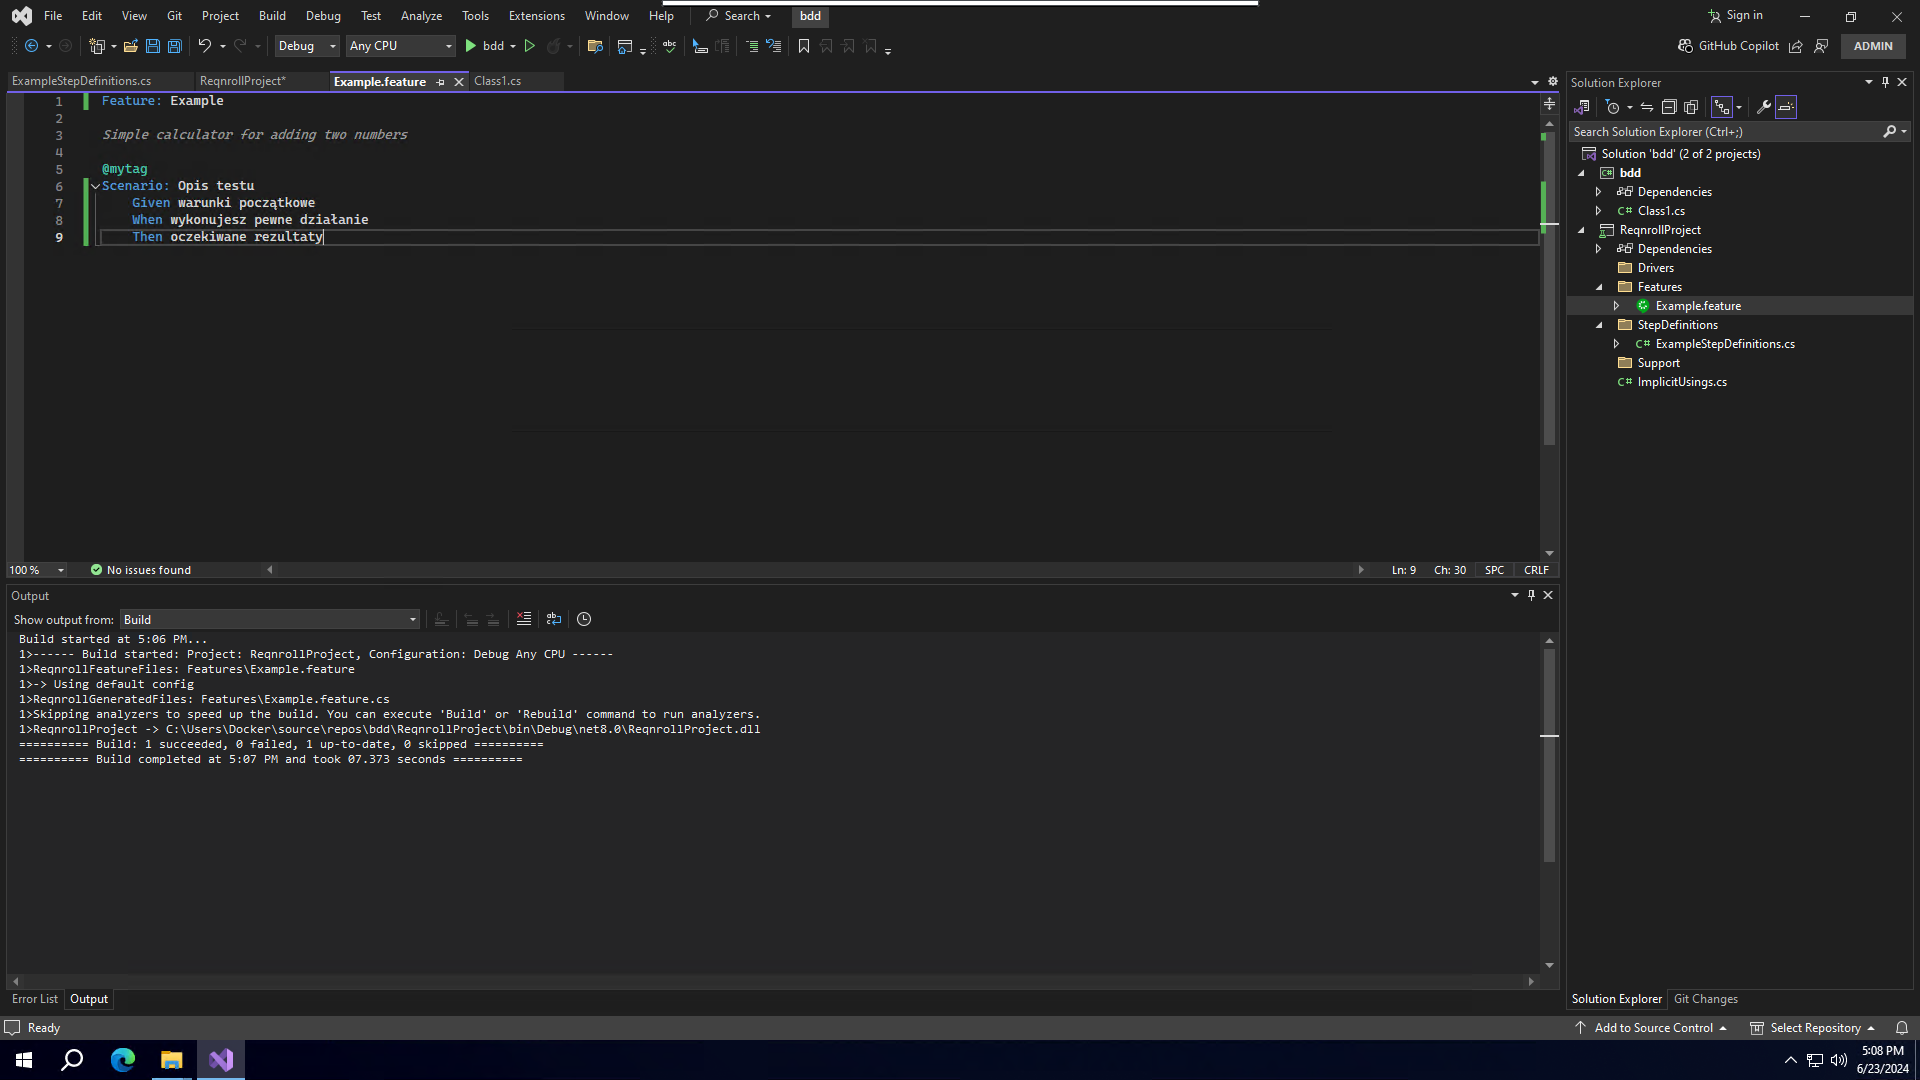
\includegraphics[width=1\textwidth,keepaspectratio]{image-23.png}
  \caption{Utworzenie przykładowego feature'a}
  \label{fig:image-23}
\end{figure}
\begin{figure}[H]
  \centering
  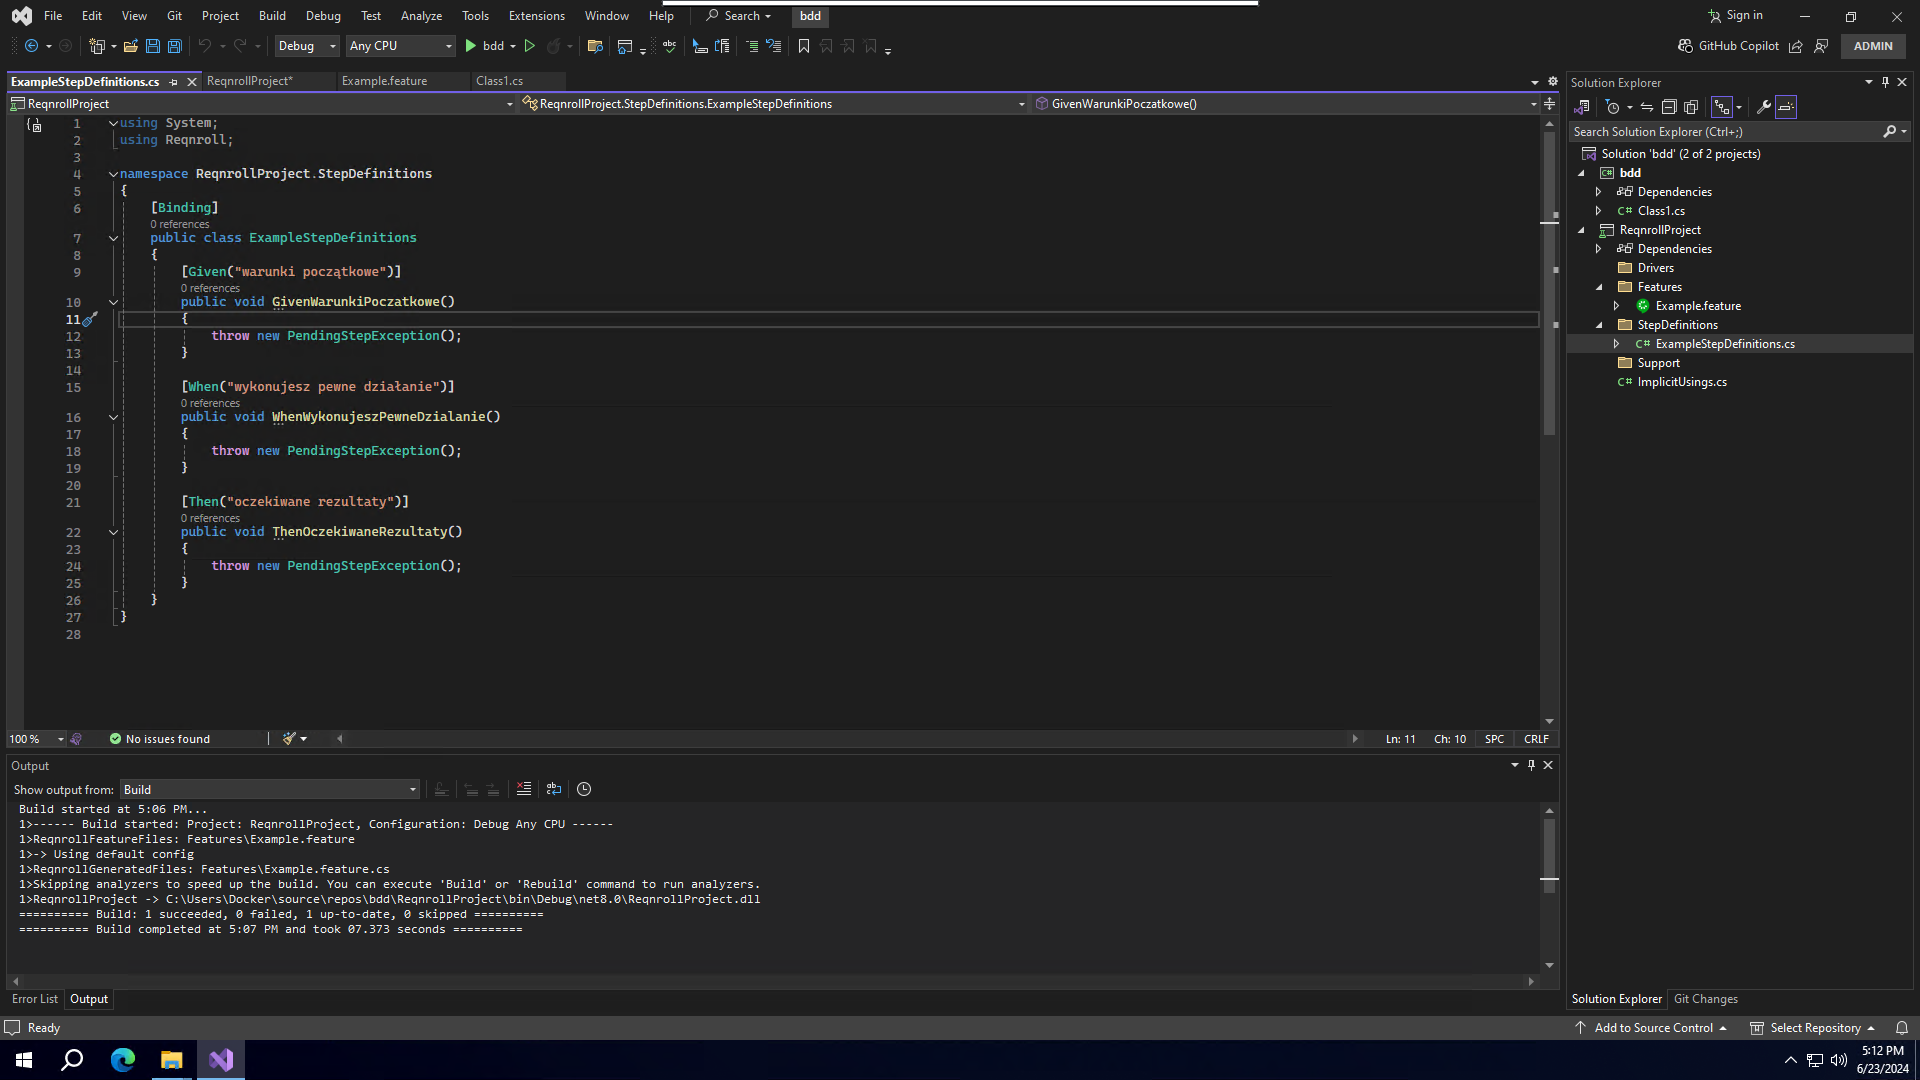
\includegraphics[width=1\textwidth,keepaspectratio]{image-24.png}
  \caption{Wygenerowanie szkieletu kodu testowego}
  \label{fig:image-24}
\end{figure}
\begin{figure}[H]
  \centering
  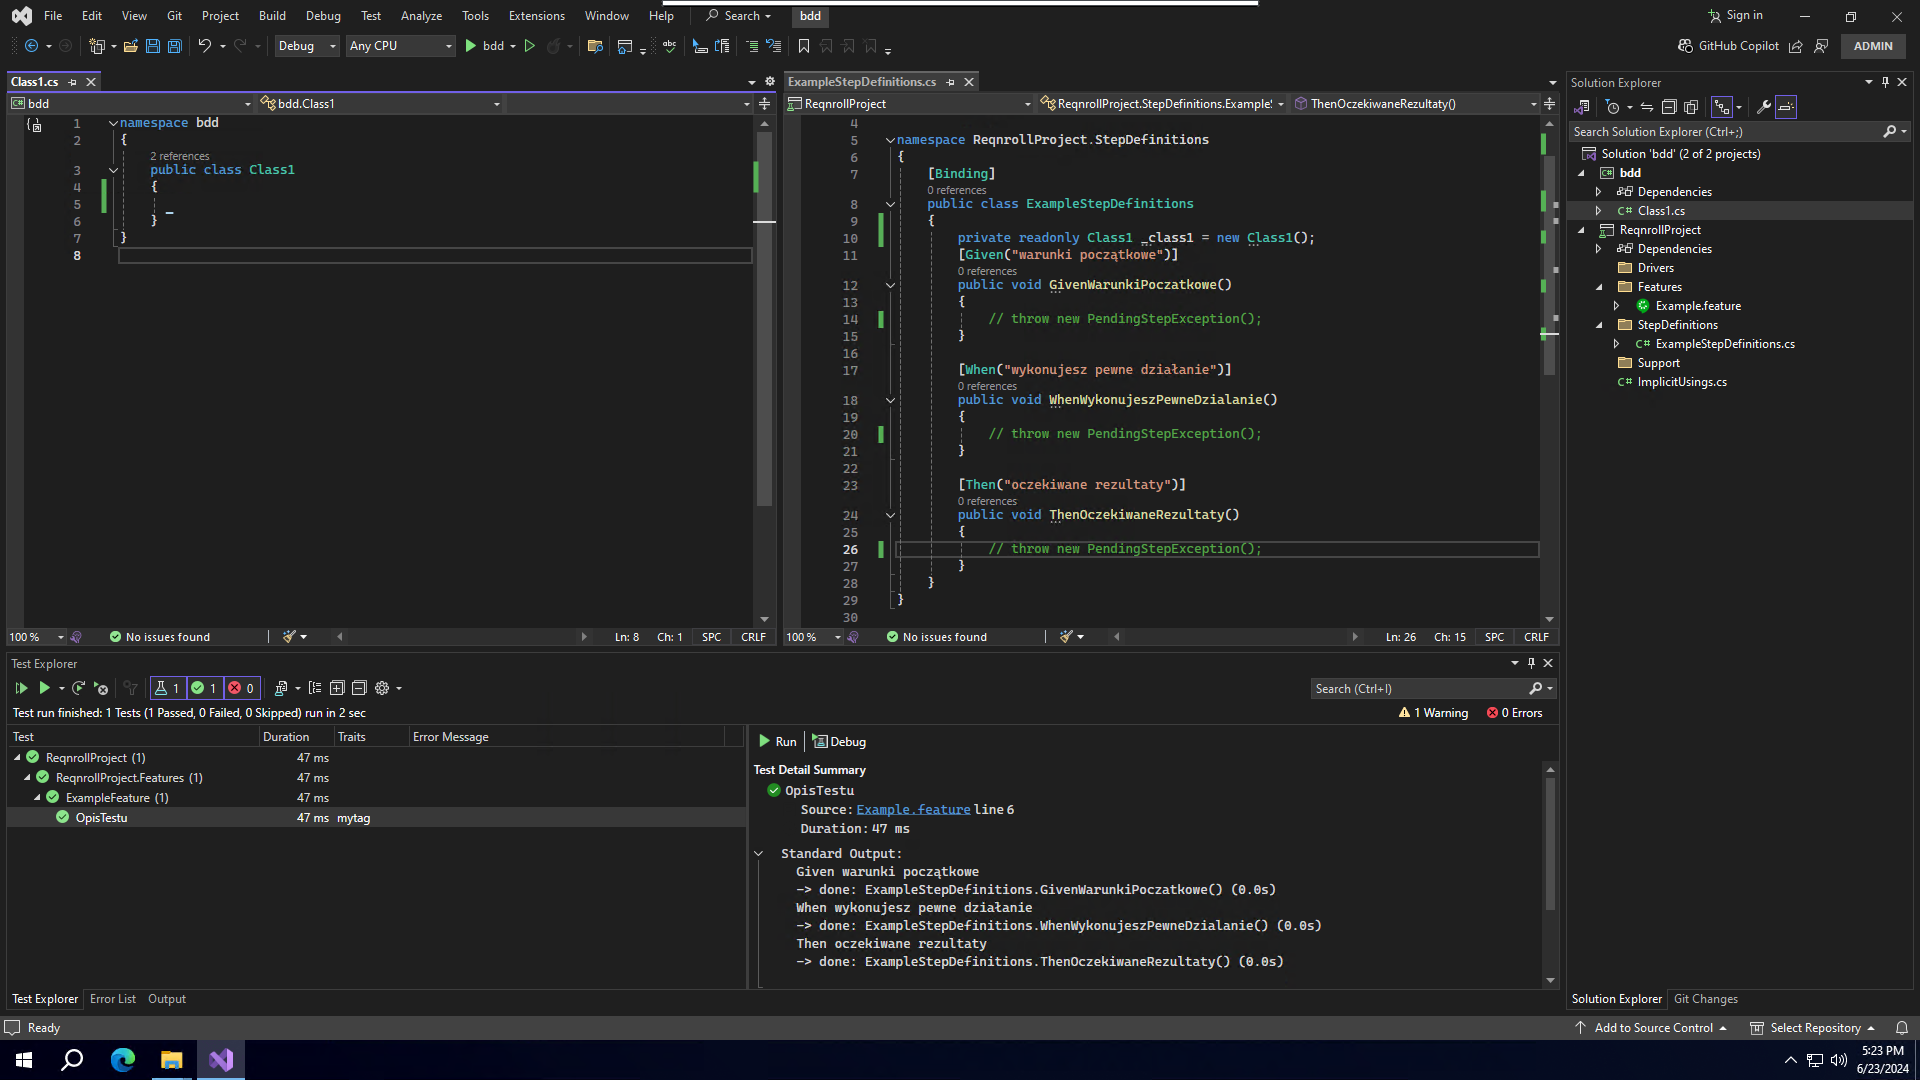
\includegraphics[width=1\textwidth,keepaspectratio]{image-25.png}
  \caption{Rezultat uruchomienia testów po skonfigurowaniu środowiska}
  \label{fig:image-25}
\end{figure}

\pagebreak
\section{Testowanie pojedynczego modułu, który jest zależny od kodu zewnętrznego.}
\begin{description}
  \item {Zastosowanie techniki symulowania zależności za pomocą biblioteki \texttt{Moq} w języku C\# umożliwia testowanie kodu korzystającego z zewnętrznych komponentów, takich jak bazy danych czy usługi sieciowe.}
\end{description}
\vspace*{\fill}
Implementacja klas \texttt{Calculator.cs} oraz \texttt{IWebService.cs}
\begin{minted}{csharp}
namespace CalculatorTests;
public interface IWebService {
    void SendData(string data);
}
\end{minted}

\begin{minted}{csharp}
namespace CalculatorTests;
public class Calculator {
    private readonly IWebService _webService;
    public Calculator(IWebService webService) {
        _webService = webService;
    }
    public int Add(int a, int b) {
        int result = a + b;
        _webService.SendData($"Add operation: {a} + {b} = {result}");
        return result;
    }
}
\end{minted}
\vspace*{\fill}
\newpage
Implementacja kodu testów

\begin{minted}{csharp}
using Xunit;
using Moq;

namespace CalculatorTests {
    public class CalculatorTests {
        [Fact]
        public void Add_ShouldSendDataToWebService() {
            // Arrange
            var webServiceMock = new Mock<IWebService>();
            var calculator = new Calculator(webServiceMock.Object);
            // Act
            int result = calculator.Add(3, 5);
            // Assert
            Assert.Equal(8, result);
            webServiceMock.Verify(ws => ws.SendData("Add operation: 3 + 5 = 8"),
            Times.Once);
        }
    }
}
\end{minted}
\begin{figure}[H]
  \centering
  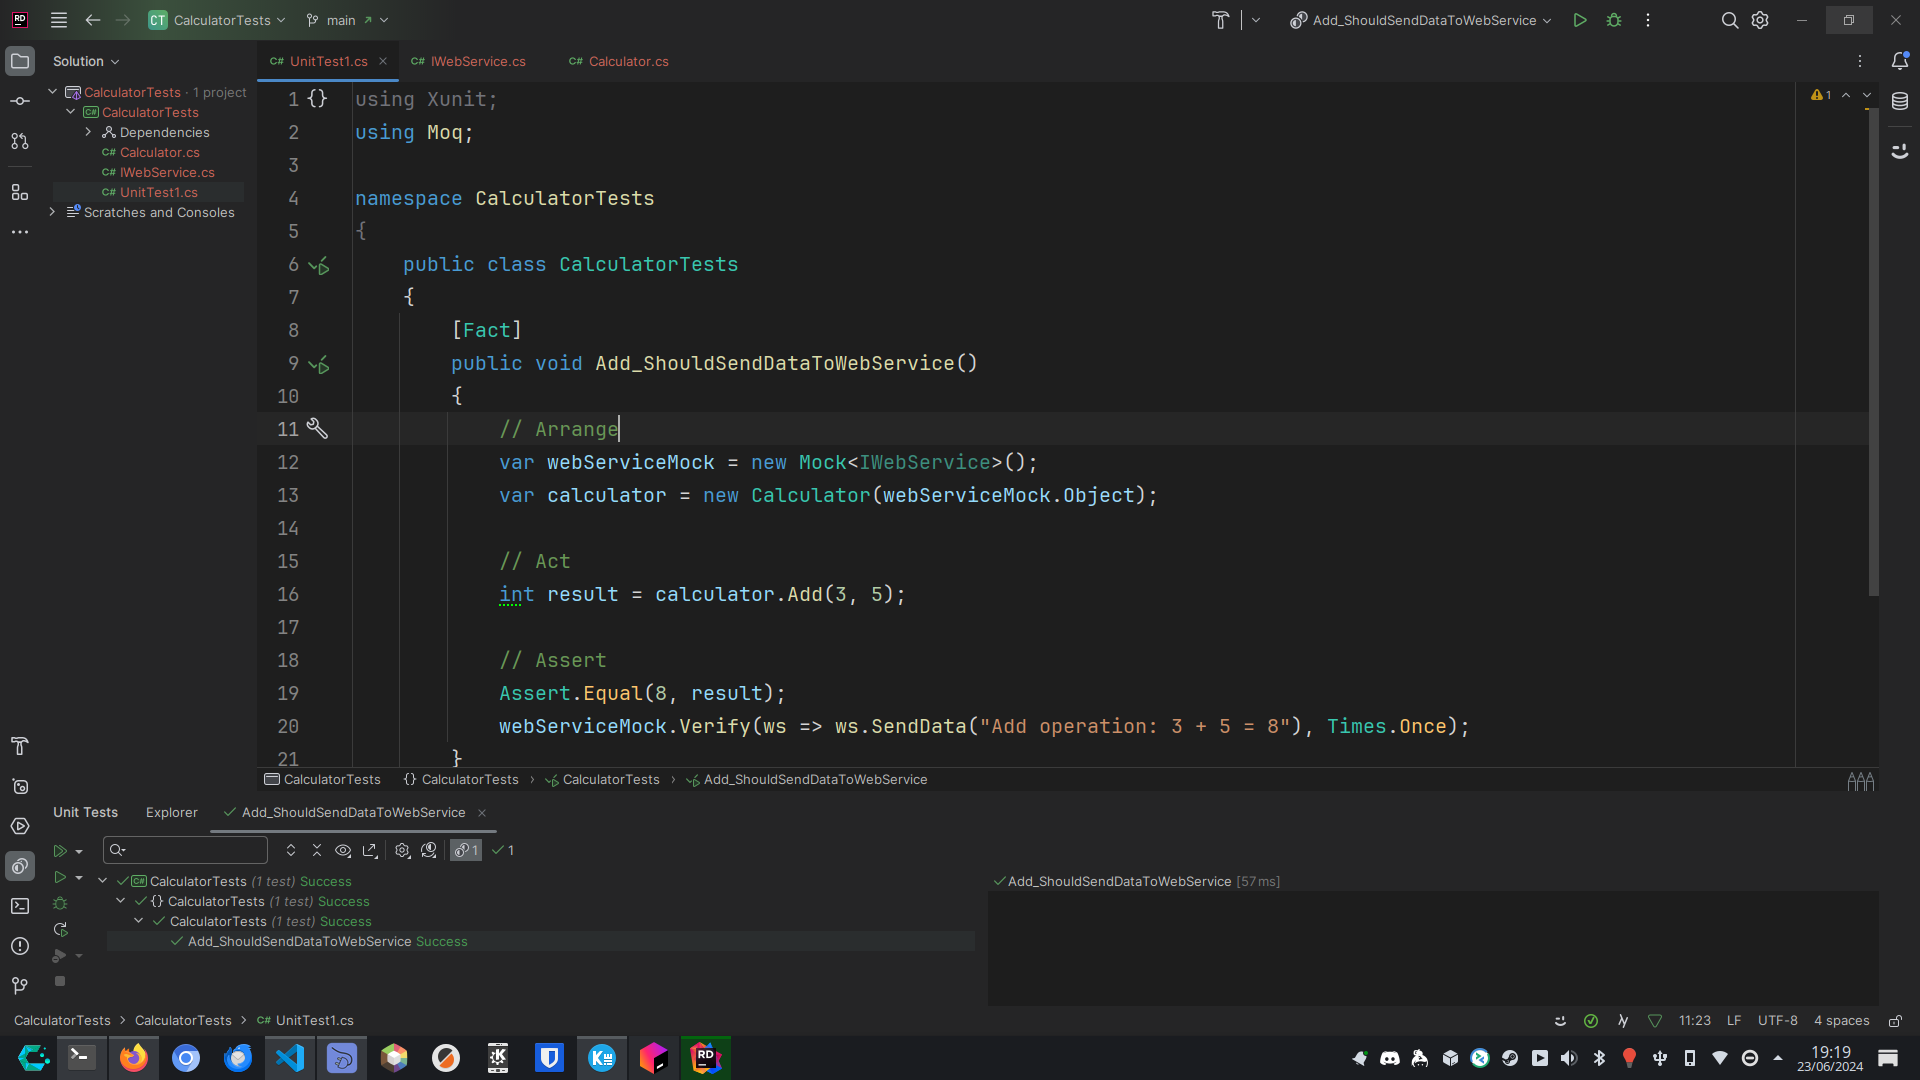
\includegraphics[width=1\textwidth,keepaspectratio]{image-26.png}
  \caption{Wynik uruchomienia testów}
  \label{fig:image-26}
\end{figure}

\pagebreak
\section{Weryfikowanie czy moduły zależne współpracują między sobą w sposób poprawny.}
\begin{description}
  \item Wykorzystanie biblioteki \texttt{Moq} w celu sprawdzenie, czy \texttt{OrderProcessor} poprawnie korzysta z \texttt{IOrderService} podczas przetwarzania zamówienia, czyli testowaniu interakcji między dwoma modułam.
  \item To podejście pozwola na dokładne przetestowanie współpracy między modułami, zapewniając jednocześnie izolację i powtarzalność testów jednostkowych.
  \item \textit{Wykorzystanie projektu z poprzedniego zadania}
\end{description}
\vspace*{\fill}
Implementacja wymaganych klas \texttt{OrderProcessor} oraz \texttt{IOrderService}
\begin{minted}{csharp}
namespace CalculatorTests;
public interface IOrderService {
    void PlaceOrder(string product, int quantity);
}
\end{minted}
\begin{minted}{csharp}
namespace CalculatorTests;
public class OrderProcessor {
    private readonly IOrderService _orderService;
    public OrderProcessor(IOrderService orderService) {
        _orderService = orderService;
    }
    public void ProcessOrder(string product, int quantity) {
        _orderService.PlaceOrder(product, quantity);
    }
}
\end{minted}
\vspace*{\fill}
\pagebreak
Implementacja kodu testów
\begin{minted}{csharp}
public class OrderProcessorTests {
    [Fact]
    public void ProcessOrder_ShouldCallPlaceOrderWithCorrectParameters() {
        // Arrange
        var orderServiceMock = new Mock<IOrderService>();
        var orderProcessor = new OrderProcessor(orderServiceMock.Object);
        // Act
        orderProcessor.ProcessOrder("ProductABC", 3);
        // Assert
        orderServiceMock.Verify(os => os.PlaceOrder("ProductABC", 3), Times.Once);
    }
    [Fact]
    public void ProcessOrder_ShouldCallPlaceOrderMultipleTimes() {
        // Arrange
        var orderServiceMock = new Mock<IOrderService>();
        var orderProcessor = new OrderProcessor(orderServiceMock.Object);
        // Act
        orderProcessor.ProcessOrder("Product1", 2);
        orderProcessor.ProcessOrder("Product2", 5);
        // Assert
        orderServiceMock.Verify(os => os.PlaceOrder("Product1", 2), Times.Once);
        orderServiceMock.Verify(os => os.PlaceOrder("Product2", 5), Times.Once);
    }
}
\end{minted}
\begin{figure}[H]
  \centering
  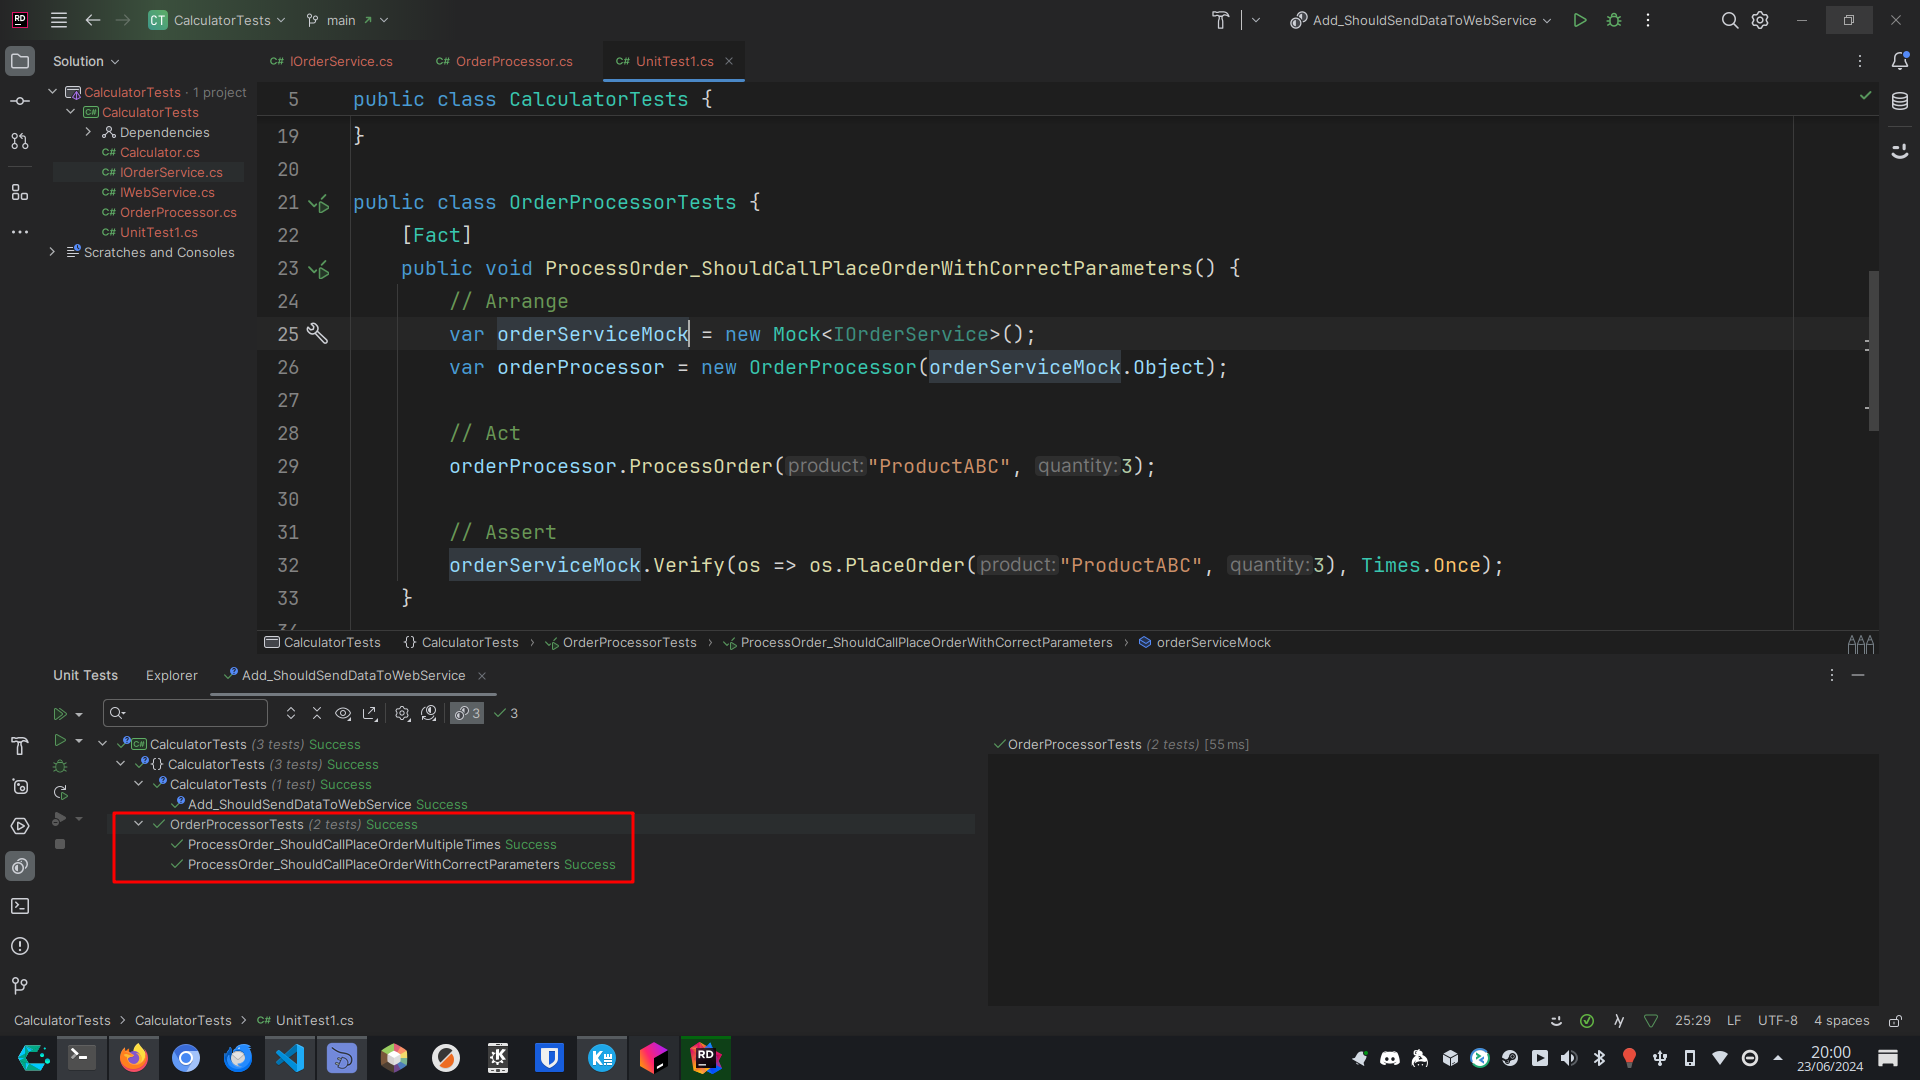
\includegraphics[width=1\textwidth,keepaspectratio]{image-27.png}
  \caption{Wynik uruchomienia testów}
  \label{fig:image-27}
\end{figure}
\end{document}
